
\section{BranchyNet Training}

%\begin{figure}
%	\centering
%	\captionsetup[subfigure]{justification=centering}
%	\subfloat[Train loss\label{fig:B-resnet-miniimagenet10-train-loss}]{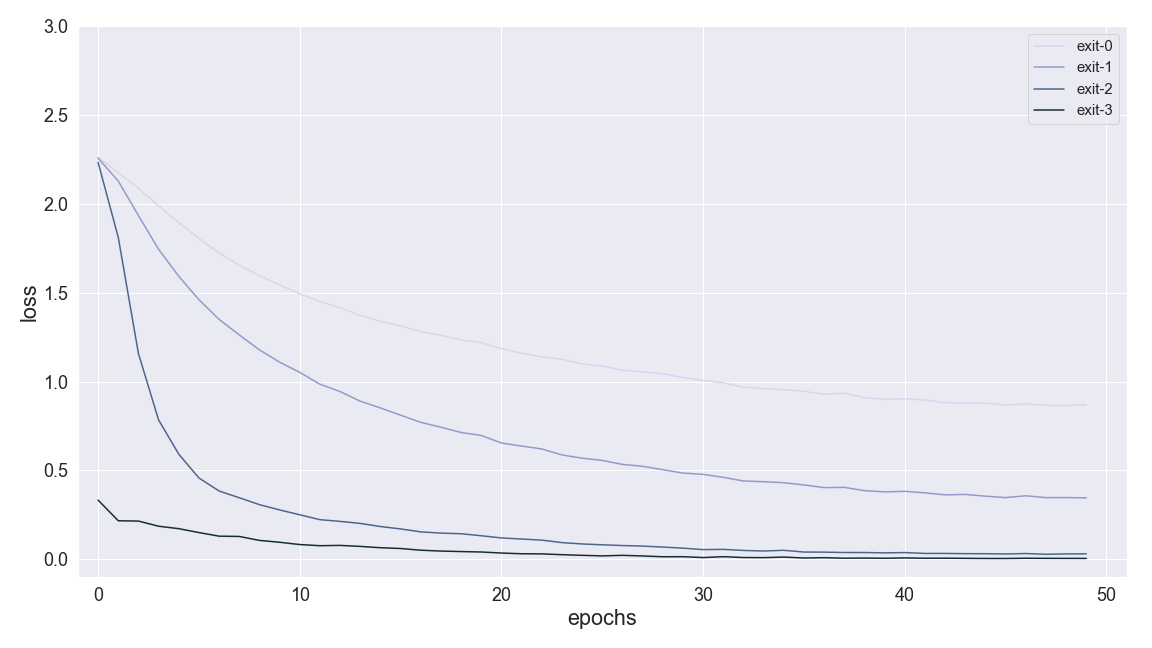
\includegraphics[width=.49\textwidth]{figures/bresnet_mini10/BResNet_train_loss_miniimagenet10.png}}
%	\subfloat[Test loss \label{fig:B-resnet-miniimagenet10-test-loss}]{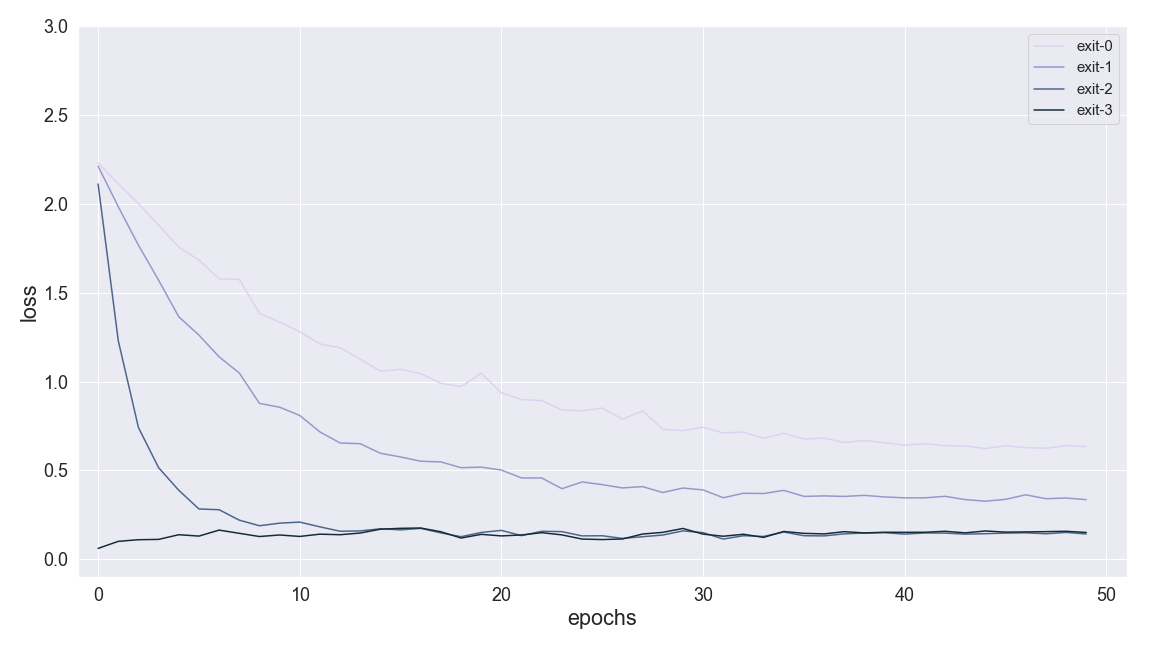
\includegraphics[width=.49\textwidth]{figures/bresnet_mini10/BResNet_test_loss_miniimagenet10.png}}
%	\hfill
%	\subfloat[Train accuracy\label{fig:B-resnet-miniimagenet10-train-acc}]{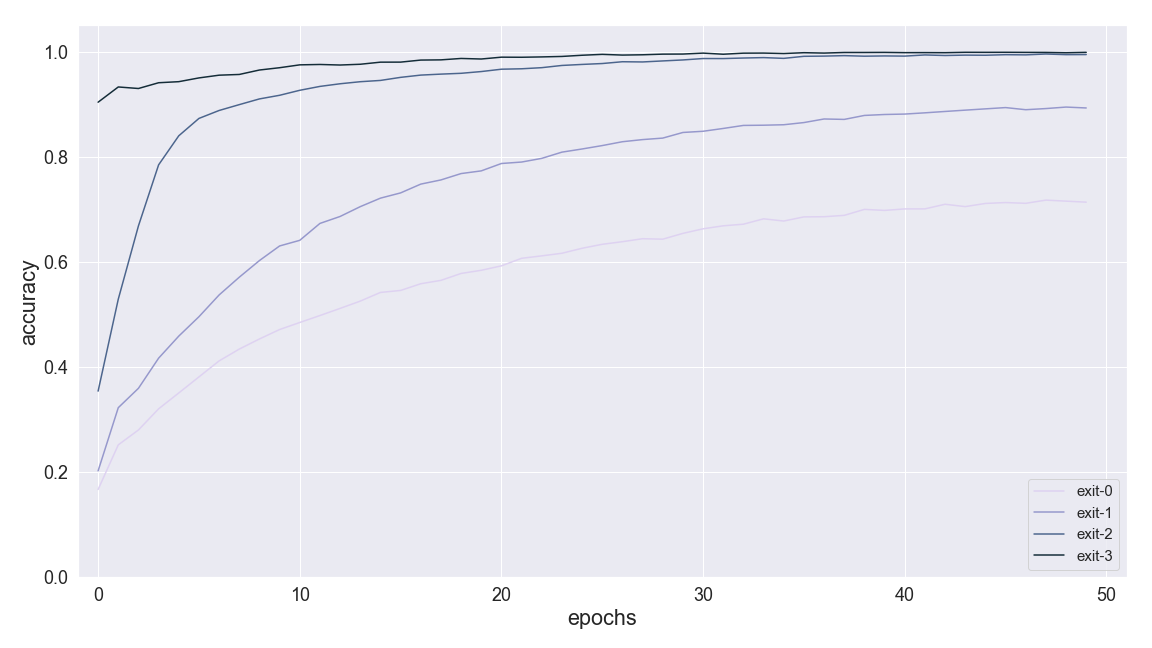
\includegraphics[width=.49\textwidth]{figures/bresnet_mini10/BResNet_train_acc_miniimagenet10.png}}
%	\subfloat[Test accuracy\label{fig:B-resnet-miniimagenet10-test-acc}]{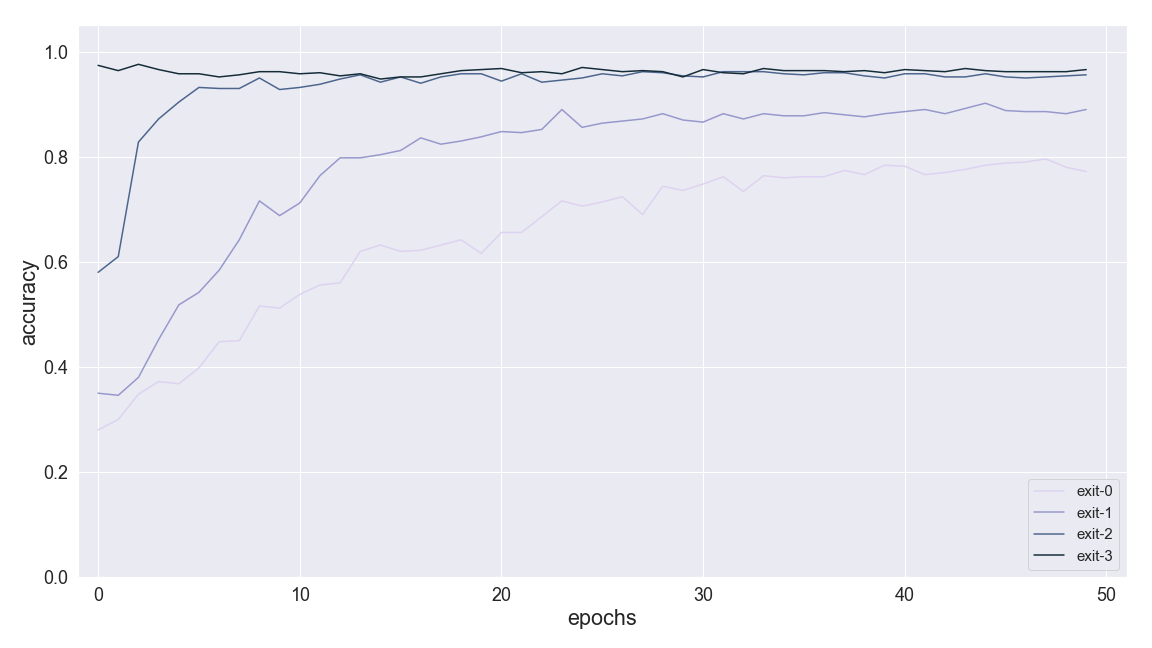
\includegraphics[width=.49\textwidth]{figures/bresnet_mini10/BResNet_test_acc_miniimagenet10.png}}
%	\caption[B-ResNet MiniImageNet10 Training summary]{Training summary shows the progression of model attributes over times of epochs, \protect\subref{fig:B-resnet-miniimagenet10-train-loss} train loss, \protect\subref{fig:B-resnet-miniimagenet10-test-loss} test loss, \protect\subref{fig:B-resnet-miniimagenet10-train-acc} train accuracy, \protect\subref{fig:B-resnet-miniimagenet10-test-acc}, test accuracy.}
%	\label{fig:B-resnet-miniimagenet-10}
%\end{figure}

Training B-\gls{resnet} and B-\gls{densenet} shows the importance of the densely connected layers for an early exiting model. The early exits of B-\gls{densenet} have a higher accuracy compared to B-\gls{resnet}, however B-\gls{resnet} last two exits are more accurate, see figure \ref{fig:b-net-miniimagenet-100}. 

\begin{figure}
	\centering
	\captionsetup[subfigure]{justification=centering}
	\subfloat[B-Resnet\label{fig:B-resnet-miniimagenet100}]{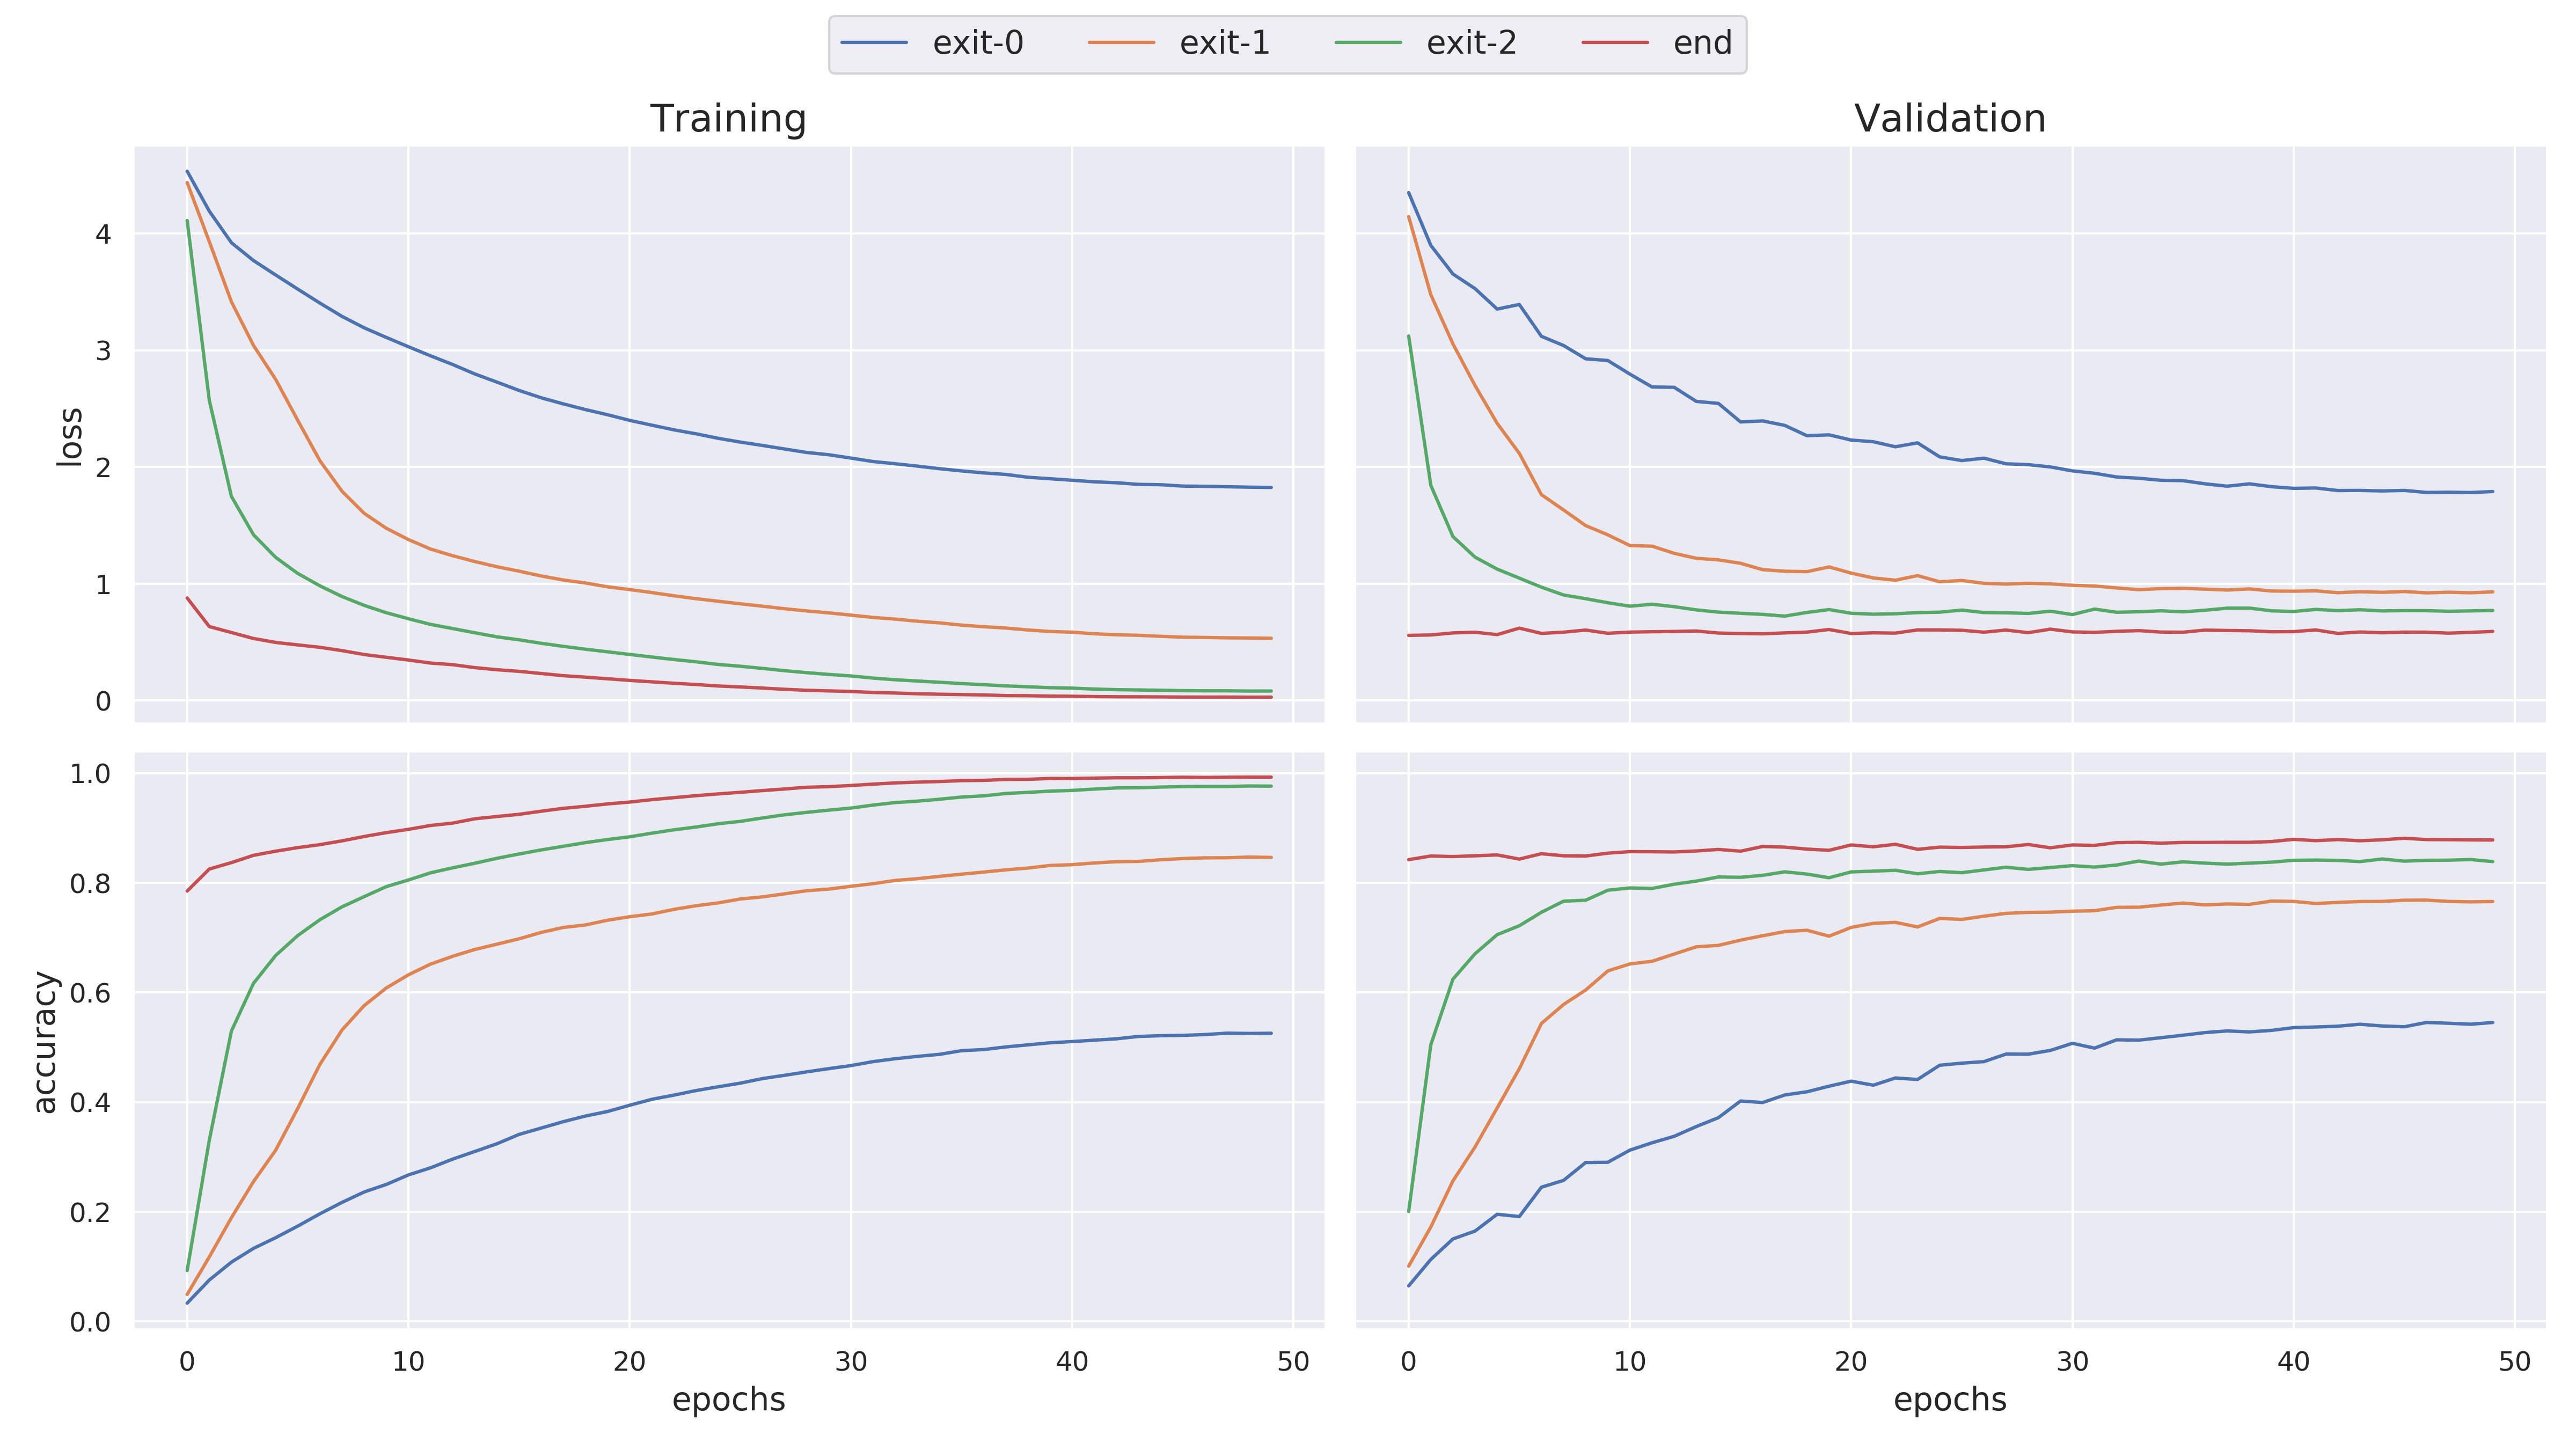
\includegraphics[width=\linewidth]{figures/training_plots/resnet_miniimagenet100}}
\end{figure}

The two last exits of \gls{resnet} are almost equally accurate. The resolution block of exit-2 are very deep, and the features becomes optimized for this classifier, hence not much gain in accuracy is obtained by running the early exit model all the way to the end. \gls{densenet} on the other hand always have an accuracy gain by continuing the inference process.    

\begin{figure}
	%\ContinuedFloat
	\captionsetup[subfigure]{justification=centering}
	\subfloat[B-DenseNet\label{fig:B-densenet-miniimagenet100}]{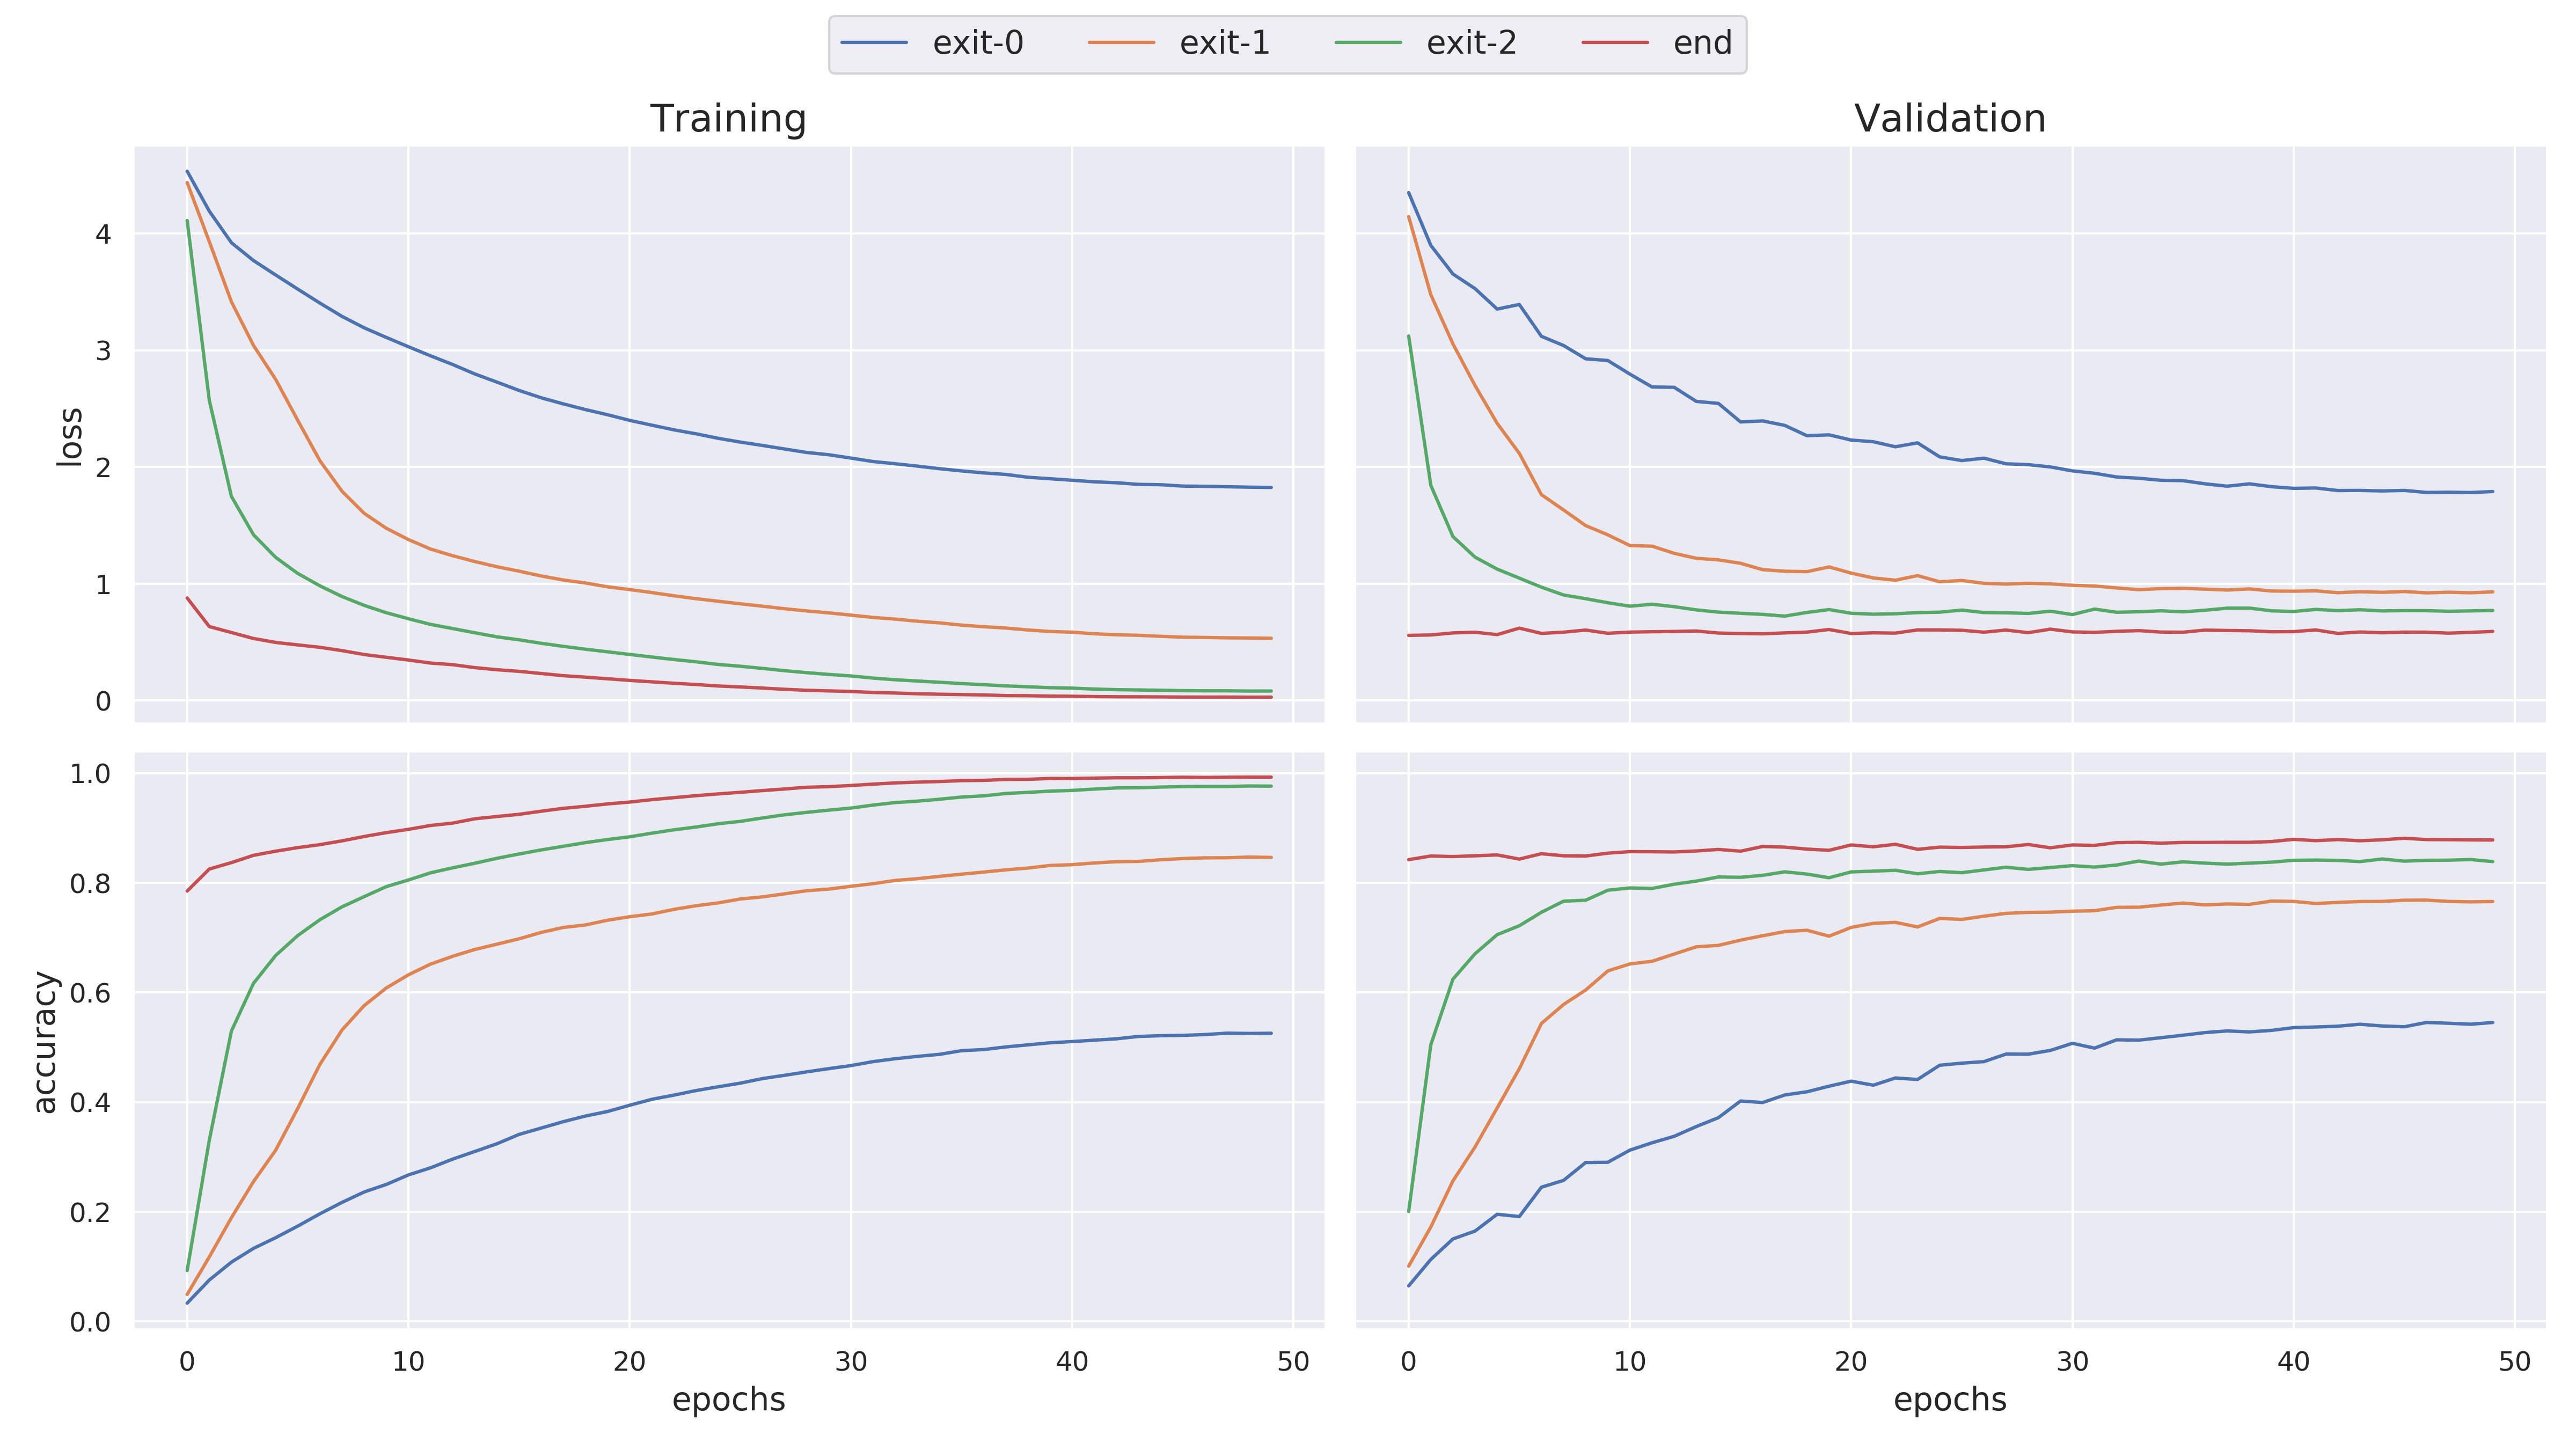
\includegraphics[width=\linewidth]{figures/training_plots/densenet_miniimagenet100}}
\end{figure}

\begin{figure}
	%\ContinuedFloat
	\captionsetup[subfigure]{justification=centering}
	\subfloat[MSDNet\label{fig:msdnet-miniimagenet100}]{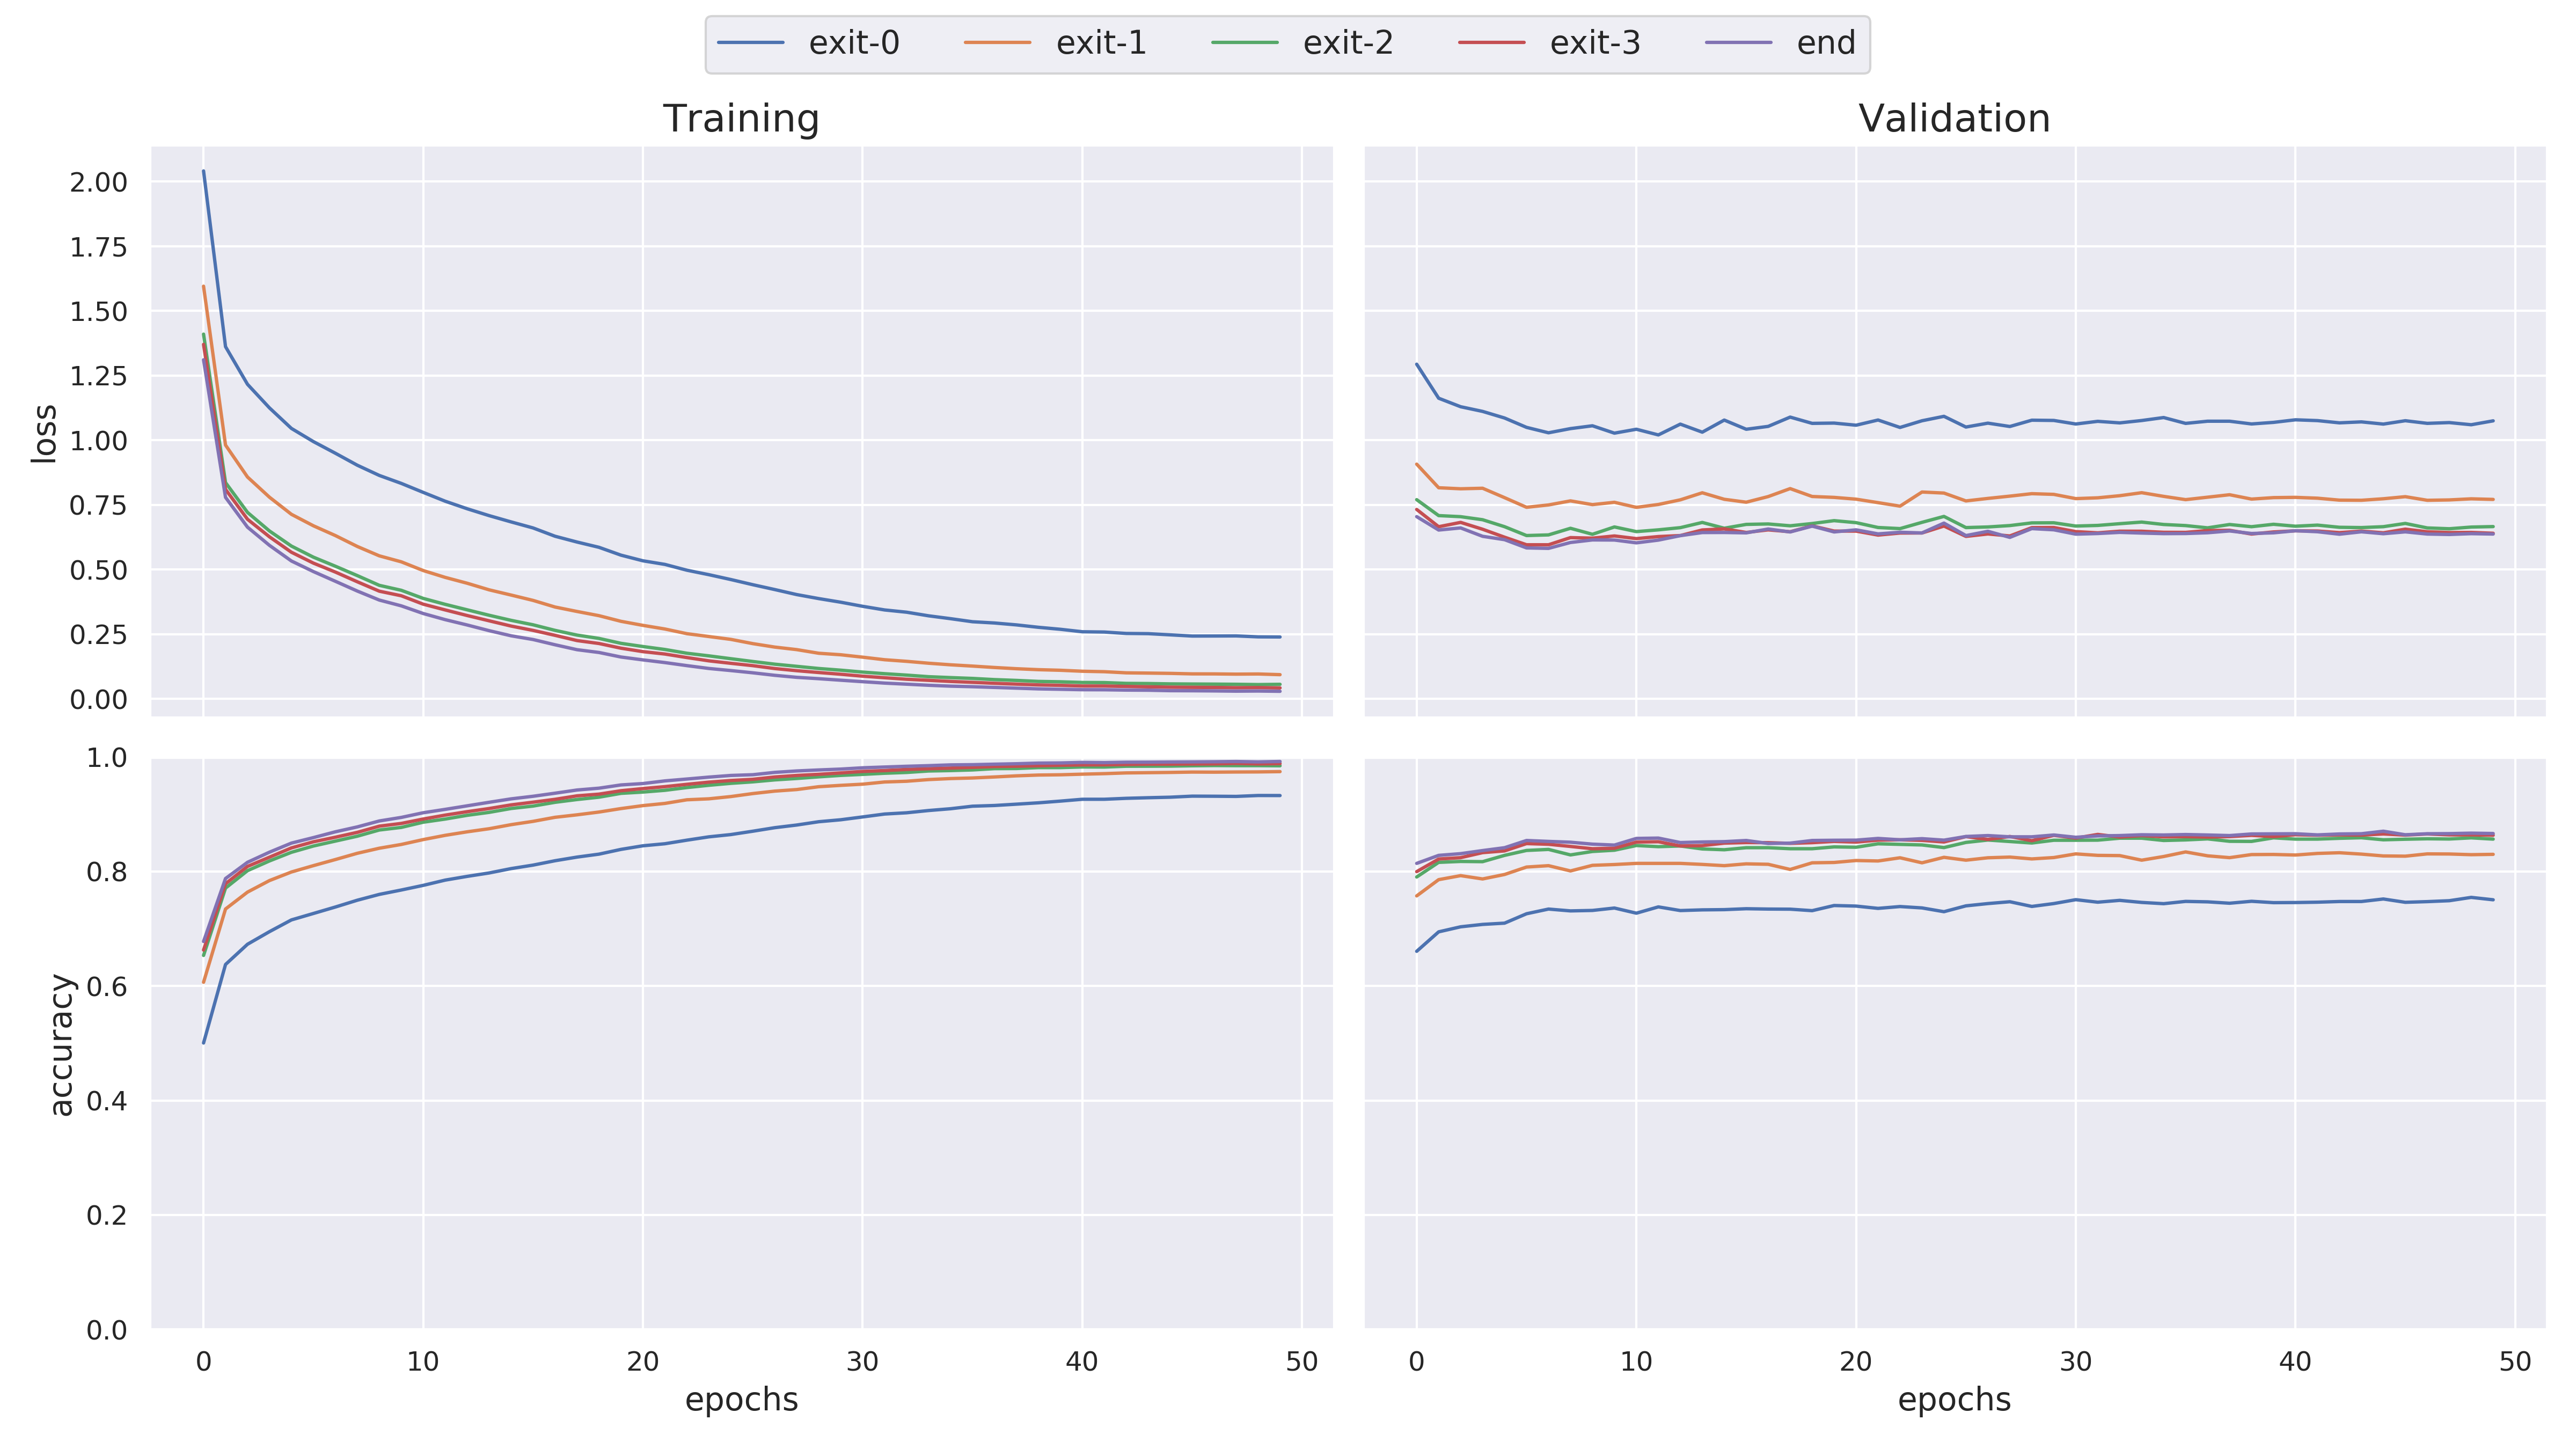
\includegraphics[width=\linewidth]{figures/training_plots/msd_miniimagenet100}}
	\caption[Training progress of BrancyNets]{Training progress for \protect\subref{fig:B-resnet-miniimagenet100} B-ResNet, \protect\subref{fig:B-densenet-miniimagenet100} B-DenseNet and \protect\subref{fig:msdnet-miniimagenet100} MSDNet} 
	\label{fig:b-net-miniimagenet-100}
\end{figure}


\section{Inference Testing}

In this test all validation samples are inferred to all three models. Each branch classifies the samples, but does not perform exit but continues the inference process. Figure \ref{fig:exit-accuracy} show the accuracy of each exit.  

\begin{figure}
	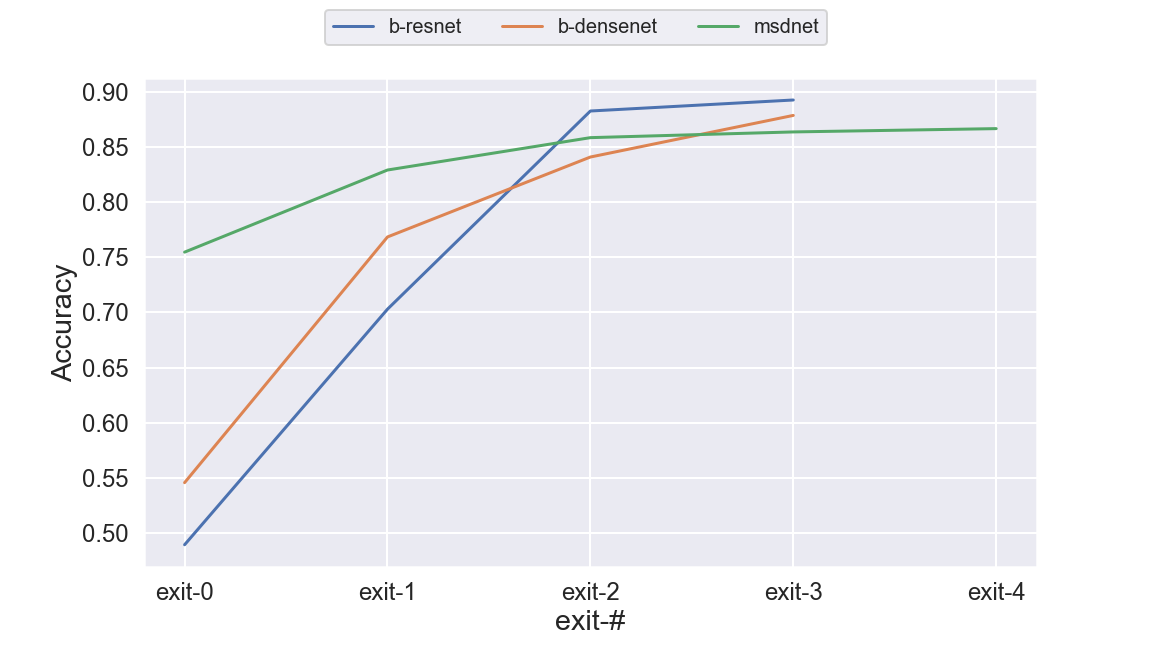
\includegraphics[width=\linewidth]{figures/inference_plots/exit_acc}
	\caption[Model Inference Accuracy]{Model Inference Accuracy}
	\label{fig:exit-accuracy}
\end{figure}

As expected the models become more accurate as we go deeper in the network. The features deep within the network have more discriminative characteristics. As stated in \cite{huang_multi-scale_2017} the densely connected features are important factors for obtaining intermediate classifiers with decent accuracy. The B-\gls{densenet} and \gls{msdnet} have as expected more accurate early classifiers, however the end-exit of B-\gls{resnet} achieves superior accuracy compared to the other models.

Still about half the samples can be accurately classified at the very first exit, which justifies the assumption for \gls{branchynet} and we can expectedly save time but let samples exit prematurely, see figure \ref{fig:exit-time}

\begin{figure}
	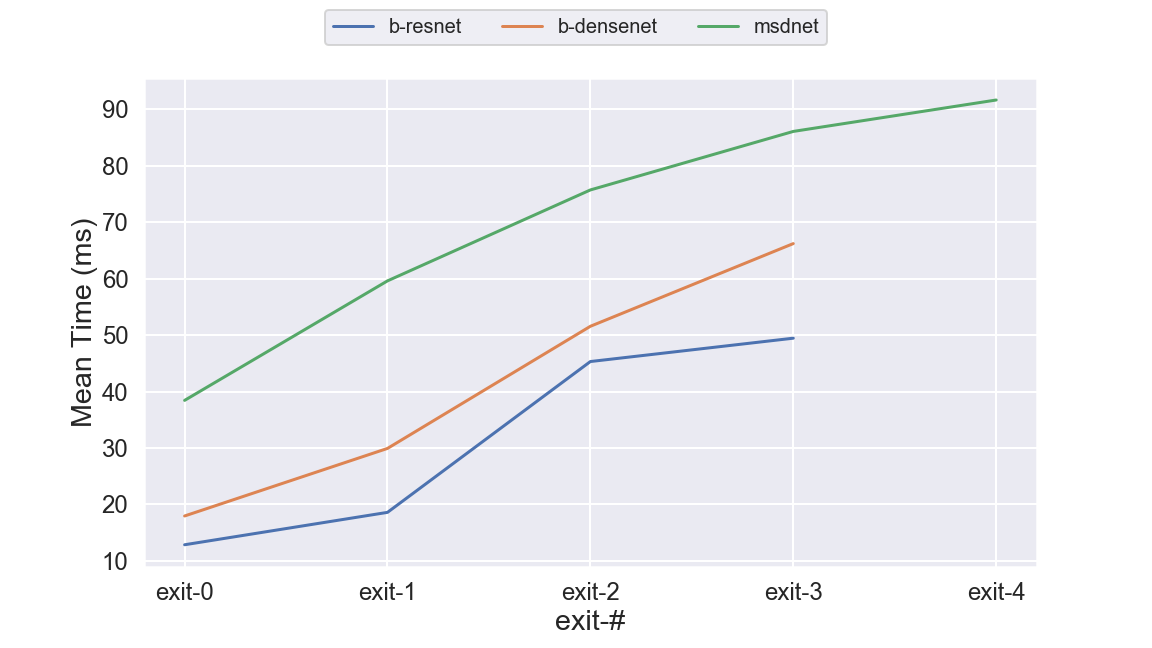
\includegraphics[width=\linewidth]{figures/inference_plots/exit_time}
	\caption[Model Inference Accuracy]{Model Inference Time}
	\label{fig:exit-time}
\end{figure}

Figure \ref{fig:exit-time} shows the average inference time for a classification at the corresponding exit. If the model decides to exit earlier in the network, the figure shows the time savings achievable. The inference time is hardware dependent and a full model comparison cannot be made solely by this test, later tests compares the inference time of the models on different platforms, however the trend seems to be, that B-\gls{resnet} is the fastest, followed by B-\gls{densenet} an lastly \gls{msdnet}. Table \ref{tbl:early-exit} shows the accuracy and mean time in tabular form.

\begin{longtabu}{>{\bfseries}X|X|X}
	\caption[Early exit models' last exit accuracy]{Early exit models' last exit accuracy}\label{tbl:early-exit} \\
	\toprule
	\rowfont{\bfseries}
	Model & Accuracy & Mean Time (ms) \tabularnewline
	\hline
	\endfirsthead
	\multicolumn{3}{@{}l}{\textbf{\textcolor{black}{Table \ref{tbl:early-exit}:}} continued}\\
	\toprule
	\rowfont{\bfseries}
	Model & Accuracy & Mean Time (ms) \tabularnewline
	\hline
	\endhead % all the lines above this will be repeated on every page
	\hline
	\multicolumn{3}{@{}l}{continued \ldots}\\
	\endfoot
	\hline
	\endlastfoot
	B-ResNet & \tabularnewline
	\hspace{3mm} Exit-0 & 0.489 & 12.87 \tabularnewline
	\hspace{3mm} Exit-1 & 0.703 & 18.61 \tabularnewline
	\hspace{3mm} Exit-2 & 0.883 & 45.31 \tabularnewline
	\hspace{3mm} Exit-3 & 0.893 & 49.45 \tabularnewline
	\hline
	B-DenseNet &  \tabularnewline
	\hspace{3mm} Exit-0 & 0.545 & 17.96 \tabularnewline
	\hspace{3mm} Exit-1 & 0.769 & 29.93 \tabularnewline
	\hspace{3mm} Exit-2 & 0.841 & 51.56 \tabularnewline
	\hspace{3mm} Exit-3 & 0.879 & 66.20 \tabularnewline
	\hline
	MSDNet & \tabularnewline
	\hspace{3mm} Exit-0 & 0.755 & 38.43 \tabularnewline
	\hspace{3mm} Exit-1 & 0.829 & 59.60 \tabularnewline
	\hspace{3mm} Exit-2 & 0.859 & 75.70 \tabularnewline
	\hspace{3mm} Exit-3 & 0.864 & 86.06 \tabularnewline
	\hspace{3mm} Exit-4 & 0.867 & 91.63 \tabularnewline
	\bottomrule
\end{longtabu}

The challenge is to known when to let samples exit, which can either be done at random or using the output from the softmax function, which can be interpreted as a confidence metric for the prediction. In the next test, we evaluate the two mentioned confidence scores as a threshold for exiting. 


%\paragraph{Pascal VOC}
%
%\begin{figure}
%	\centering
%	\captionsetup[subfigure]{justification=centering}
%	\subfloat[Train loss\label{fig:B-resnet-voc-train-loss}]{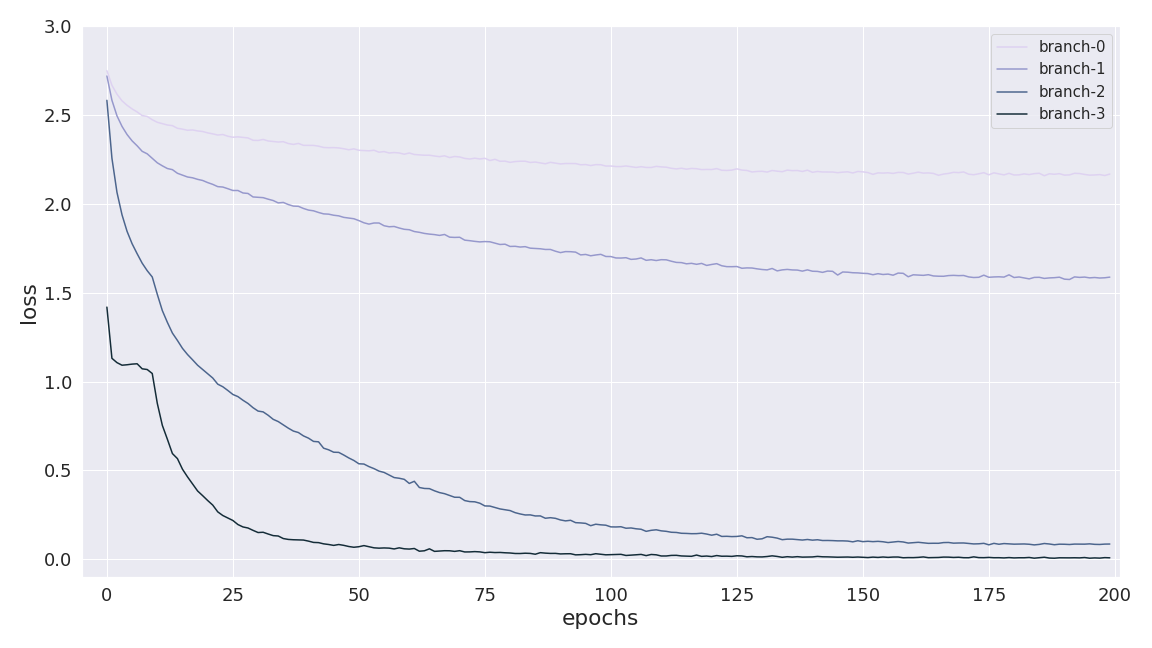
\includegraphics[width=.49\textwidth]{figures/BResNetVOC/BResNet_train_loss_VOC.png}}
%	\subfloat[Test loss \label{fig:B-resnet-voc-test-loss}]{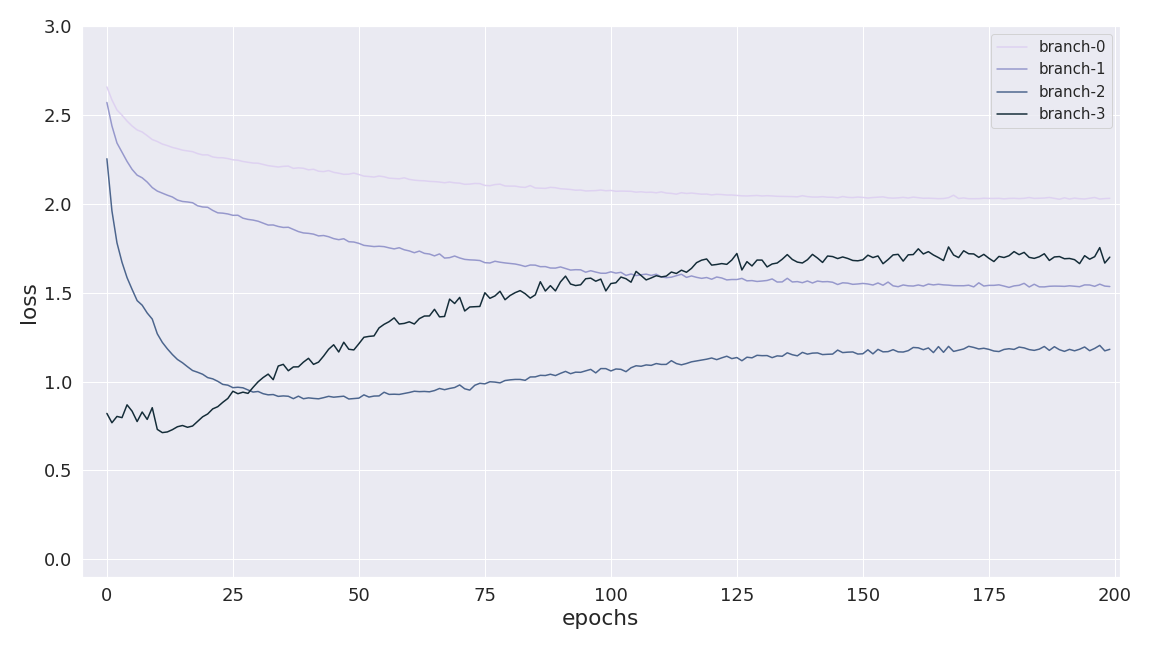
\includegraphics[width=.49\textwidth]{figures/BResNetVOC/BResNet_test_loss_VOC.png}}
%	\hfill
%	\subfloat[Train accuracy\label{fig:B-resnet-voc-train-acc}]{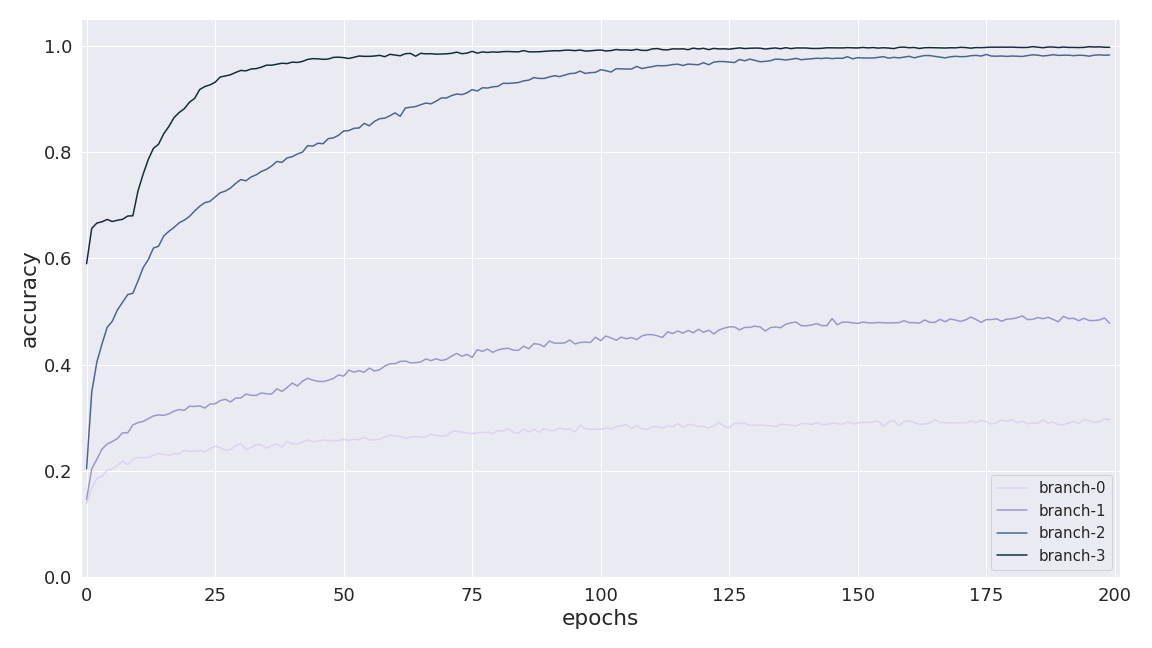
\includegraphics[width=.49\textwidth]{figures/BResNetVOC/BResNet_train_acc_VOC.png}}
%	\subfloat[Test accuracy\label{fig:B-resnet-voc-test-acc}]{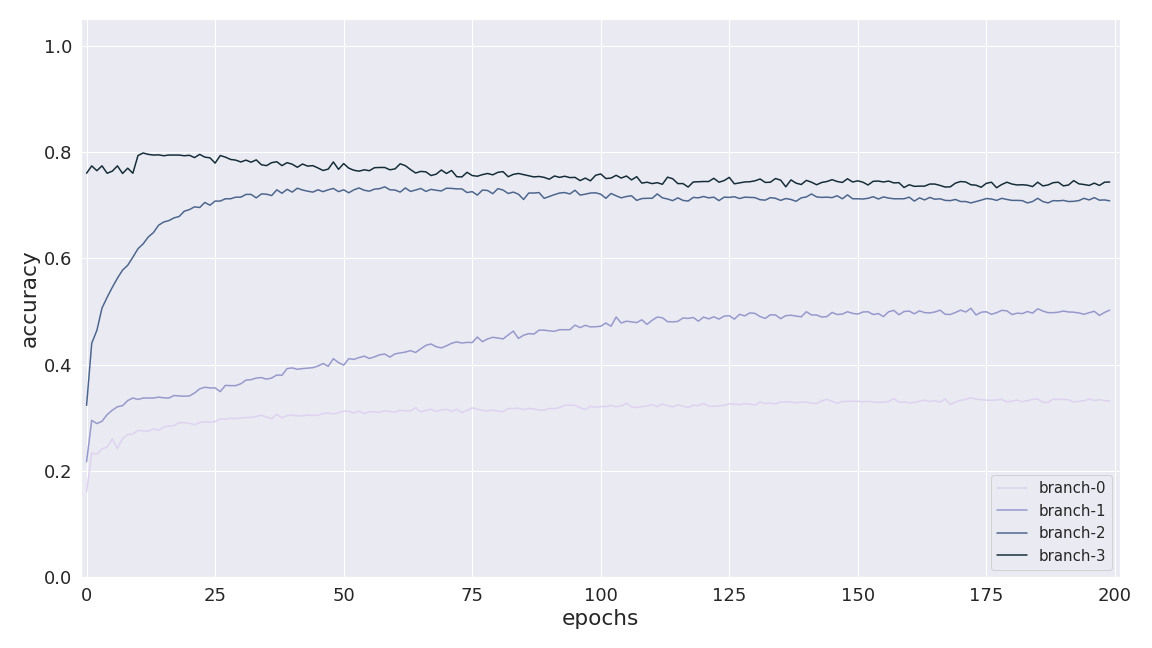
\includegraphics[width=.49\textwidth]{figures/BResNetVOC/BResNet_test_acc_VOC.png}}
%	\caption[B-ResNet VOC Training summary]{Training summary shows the progression of model attributes over times of epochs, \protect\subref{fig:B-resnet-voc-train-loss} train loss, \protect\subref{fig:B-resnet-voc-test-loss} test loss, \protect\subref{fig:B-resnet-voc-train-acc} train accuracy, \protect\subref{fig:B-resnet-voc-test-acc}, test accuracy.}
%\end{figure}
%
%Visualizing the training progression, clearly indicates that model overfitting to the training data. When a model overfits it suffers to generalize the true underlying distribution of the data. This can be caused by insufficient number of training samples or too complex a model. Since the model has shown promising results in image classification task previously, we can conclude, that the dataset is too sparse.
%
%Even though the model fails to generalize, the experiment still produce interesting results. Given an early exiting model as B-ResNet 50\% of the test samples can be correctly classified using only half of the \gls{dnn}.


\section{Threshold Analysis}

In this experiment the MiniImageNet100 validation set have been used to evaluate the two threshold metrics; \emph{Confidence Threshold} and \emph{Score-Margin Threshold}. \Cref{fig:resnet_confidence,fig:resnet_score-margin,fig:densenet_confidence,fig:densenet_score-margin,fig:msdnet_confidence,fig:msdnet_score-margin} compares the performance of each exit on all samples. The figures show for each of the three networks under test a plot of the two thresholds for all exit for the model. It shows the frequency of exited samples, that have been correctly classified ({\color{sns-green}green}) and incorrectly classified ({\color{sns-red}red}). As well as, samples that could not be classified with proper confidence given the threshold metric, hence not exited at the exit ({\color{sns-blue}blue}). Along with a plot of the change in accuracy for the exit as the confidence grows ({\color{sns-orange}orange}).  

\newcounter{imagenumber}
\begin{minipage}{\textwidth}
\begin{figure}
	\centering
	\paragraph{B-ResNet}
	
\includegraphics[width=\linewidth]{figures/threshold_plots/threshold_analysis_legend}
\end{figure}

\begin{minipage}{0.5\textwidth}
	\begin{figure}
		\captionsetup[subfloat]{farskip=1pt,captionskip=1pt, justification=centering}
		\centering
		\forloop{imagenumber}{0}{\value{imagenumber} < 4}{
			
			\subfloat[Exit-\arabic{imagenumber}\label{fig:confidence_resnet_exit_\arabic{imagenumber}}]{\includegraphics[width=.9\linewidth]{figures/threshold_plots/threshold_analysis_b-resnet_confidence_\arabic{imagenumber}}}
			\hfill
		}
		\caption[ResNet Confidence Threshold]{Confidence Threshold}
		\label{fig:resnet_confidence}
	\end{figure}
\end{minipage}
\begin{minipage}{0.5\textwidth}
	\begin{figure}
		\captionsetup[subfloat]{farskip=1pt,captionskip=1pt, justification=centering}
		\centering
		\forloop{imagenumber}{0}{\value{imagenumber} < 4}{
			
			\subfloat[Exit-\arabic{imagenumber}\label{fig:score-margin_resnet_exit_\arabic{imagenumber}}]{\includegraphics[width=.9\linewidth]{figures/threshold_plots/threshold_analysis_b-resnet_score-margin_\arabic{imagenumber}}}
			\hfill
		}
		\caption[ResNet Score-margin Threshold]{Score-margin Threshold}
		\label{fig:resnet_score-margin}
	\end{figure}
\end{minipage}
\end{minipage}

\begin{minipage}{\textwidth}
	\begin{figure}
		\centering
		\paragraph{B-DenseNet}
	\end{figure}
	\begin{minipage}{0.5\textwidth}
		\begin{figure}
			\captionsetup[subfloat]{farskip=1pt,captionskip=1pt, justification=centering}
			\centering
			\forloop{imagenumber}{0}{\value{imagenumber} < 4}{
				
				\subfloat[Exit-\arabic{imagenumber}\label{fig:confidence_dense_exit_\arabic{imagenumber}}]{\includegraphics[width=.9\linewidth]{figures/threshold_plots/threshold_analysis_b-densenet_confidence_\arabic{imagenumber}}}
				\hfill
			}
			\caption[DenseNet Confidence Threshold]{Confidence Threshold}
			\label{fig:densenet_confidence}
		\end{figure}
	\end{minipage}
	\begin{minipage}{0.5\textwidth}
		\begin{figure}
			\captionsetup[subfloat]{farskip=1pt,captionskip=1pt, justification=centering}
			\centering
			\forloop{imagenumber}{0}{\value{imagenumber} < 4}{
				
				\subfloat[Exit-\arabic{imagenumber}\label{fig:score-dense_resnet_exit_\arabic{imagenumber}}]{\includegraphics[width=.9\linewidth]{figures/threshold_plots/threshold_analysis_b-densenet_score-margin_\arabic{imagenumber}}}
				\hfill
			}
			\caption[DenseNet Score-margin Threshold]{Score-margin Threshold}
			\label{fig:densenet_score-margin}
		\end{figure}
	\end{minipage}
\end{minipage}

\noindent\makebox[\textwidth][c]{\begin{minipage}{0.9\textwidth}
	\begingroup
	\leftskip=0cm plus 0.5fil \rightskip=0cm plus -0.5fil
	\parfillskip=0cm plus 1fil
	\paragraph{MSDNet}\par
	\endgroup
	
	\begin{minipage}{0.5\textwidth}
		\begin{figure}
			\captionsetup[subfloat]{farskip=0pt,captionskip=0pt, justification=centering}
			\centering
			\forloop{imagenumber}{0}{\value{imagenumber} < 5}{
				
				\subfloat[Exit-\arabic{imagenumber}\label{fig:confidence_msd_exit_\arabic{imagenumber}}]{\includegraphics[width=.9\linewidth]{figures/threshold_plots/threshold_analysis_msdnet_confidence_\arabic{imagenumber}}}
				\hfill
			}
			\caption[MSDNet Confidence Threshold]{Confidence Threshold}
			\label{fig:msdnet_confidence}
		\end{figure}
	\end{minipage}
	\begin{minipage}{0.5\textwidth}
		\begin{figure}
			\captionsetup[subfloat]{farskip=1pt,captionskip=1pt, justification=centering}
			\centering
			\forloop{imagenumber}{0}{\value{imagenumber} < 5}{
				
				\subfloat[Exit-\arabic{imagenumber}\label{fig:score-msdnet_exit_\arabic{imagenumber}}]{\includegraphics[width=.9\linewidth]{figures/threshold_plots/threshold_analysis_msdnet_score-margin_\arabic{imagenumber}}}
				\hfill
			}
			\caption[MSDNet Score-margin Threshold]{Score-margin Threshold}
			\label{fig:msdnet_score-margin}
		\end{figure}
	\end{minipage}
\end{minipage}}

The aim is to find the metric, that reduces the amount of incorrectly exited samples ({\color{sns-red}red}). Whenever samples are exited incorrectly, the overall accuracy of the models are reduced, if it could have been correctly classifed at later exit. The growing frequency of correctly exited samples ({\color{sns-green}green}) at later exits shows exactly this. As the threshold requirements are raised, it results in a higher accuracy for the exit, as the ratio between correctly exited and incorrectly exited grows. Even though all samples will be classified at the last exit, hence no sample is in fact exited at this last exit, still it shows the frequency of samples, that could not reach a confident score for the last exit. This means the accuracy for the last exit is not entirely correct.  Table \ref{tbl:early-exit} shows the accuracy of the exit, when all samples are exited at the exit. 

Generally \emph{score-margin} has more desirable traits, as less samples are incorrectly exited (red), only at the expense of a few additional samples not exited ({\color{sns-blue}blue}). The results matches \cite{park_big/little_2015}, which show a stronger correlation to actually being able to correctly predict samples given the \emph{score-margin threshold}. Henceforth the \emph{score-margin threshold} are used.

The former test is conducted b stamping all samples whether it could have been exited at the exited and if would have been correct or not. The test does not take into account if samples have been exited, then not reaching a later exit, if a exit is very confident yet incorrect. In the next test, this is accommodated for.

\begin{figure}
	\centering
	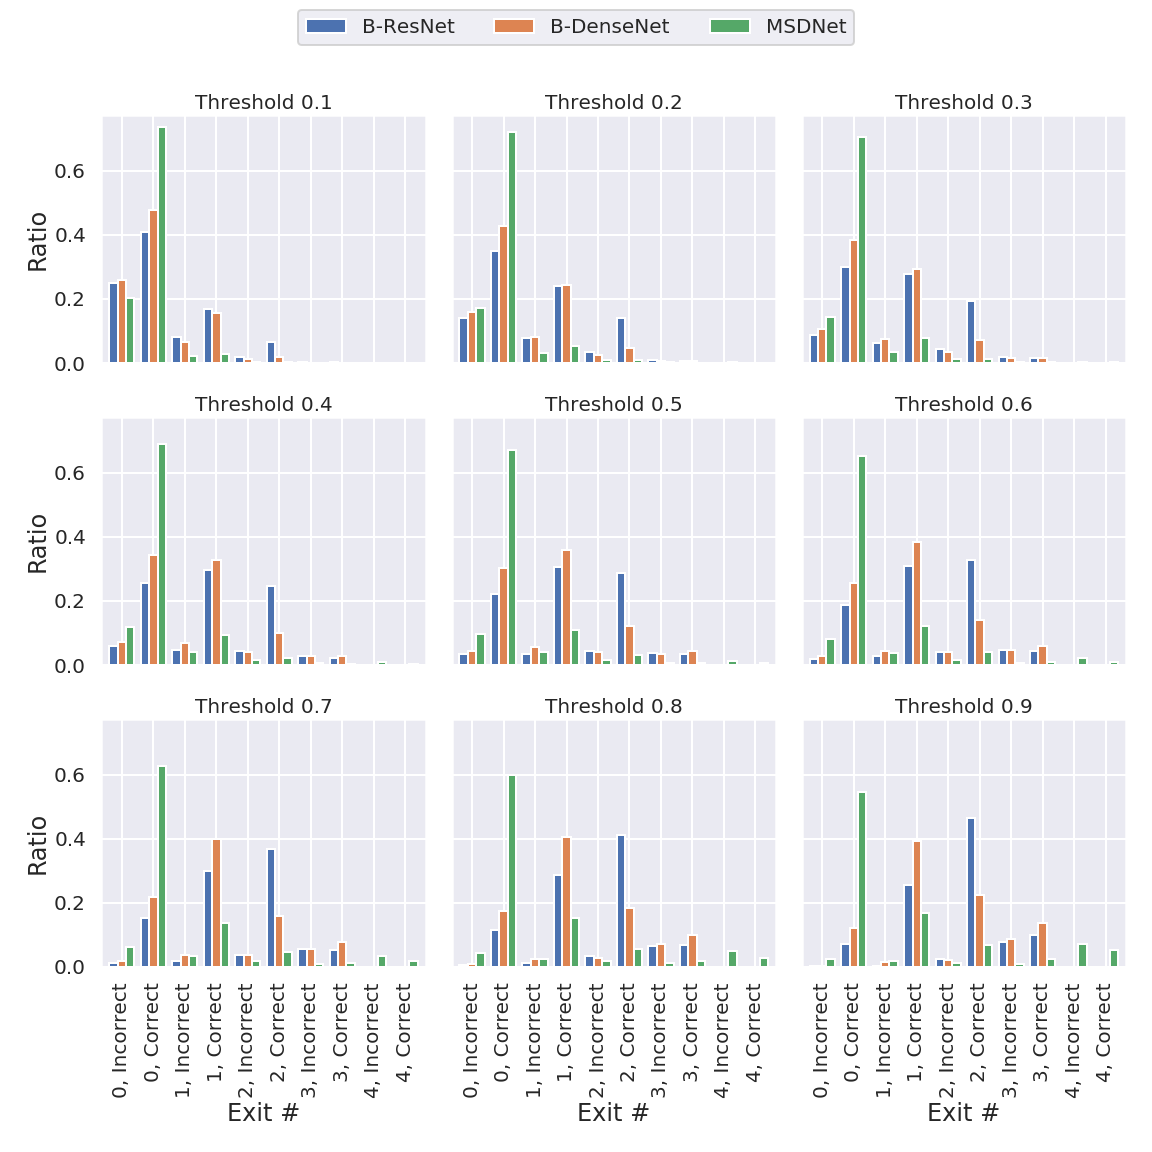
\includegraphics[width=\linewidth]{figures/threshold_plots/inference_threshold_test}
	\caption{Score-Margin Exiting}
	\label{fig:inferencethresholdtest}
\end{figure}



\section{Early Exiting vs. Conventional Inference}

Conventional versions of the \gls{resnet} and \gls{densenet} were trained on the \gls{min100}. Transfer learning was used with ImageNet weights, the model are used as a feature extractor, hence all weights were frozen and only the linear classifier was trained. The conventional models were used to compare with early exiting inference accuracy and latency on X different platforms.


\begin{longtabu}{>{\bfseries}X|X|X|X}
	\caption[Platform hardware comparison]{Platform hardware comparison of Window 10 Stationary PC and NVIDIA Jetson TX2 Edge Computer} \label{tbl:platforms} \\
	\toprule
	\rowfont{\bfseries}
	Platform & CPU & GPU & RAM  \tabularnewline
	\bottomrule
	\endfirsthead
	\multicolumn{3}{@{}l}{\textbf{\textcolor{black}{Table \ref{tbl:platforms}:}} continued}\\
	\toprule
	\rowfont{\bfseries}
	Platform & CPU & GPU & RAM  \tabularnewline
	\bottomrule
	\endhead % all the lines above this will be repeated on every page
	\bottomrule
	\multicolumn{3}{@{}l}{continued \ldots}\\
	\endfoot
	\hline
	\endlastfoot
	Windows PC & Intel i5 & NVIDIA GeForce GTX 1080, 2560 CUDA cores & 16GB \tabularnewline
	\hline
	Jetson TX2 & ARM Cortex-A57 & NVIDIA Pascal GPU, 256 CUDA cores & 8GB \tabularnewline
	\bottomrule
\end{longtabu}

The model inference characteristic on PC, see figure \ref{fig:early_exit_vs_conv}.

  \begin{figure}
  	\captionsetup[subfigure]{justification=centering}
  	\centering
  	\subfloat[Window PC\label{fig:early_exit_vs_conv}]{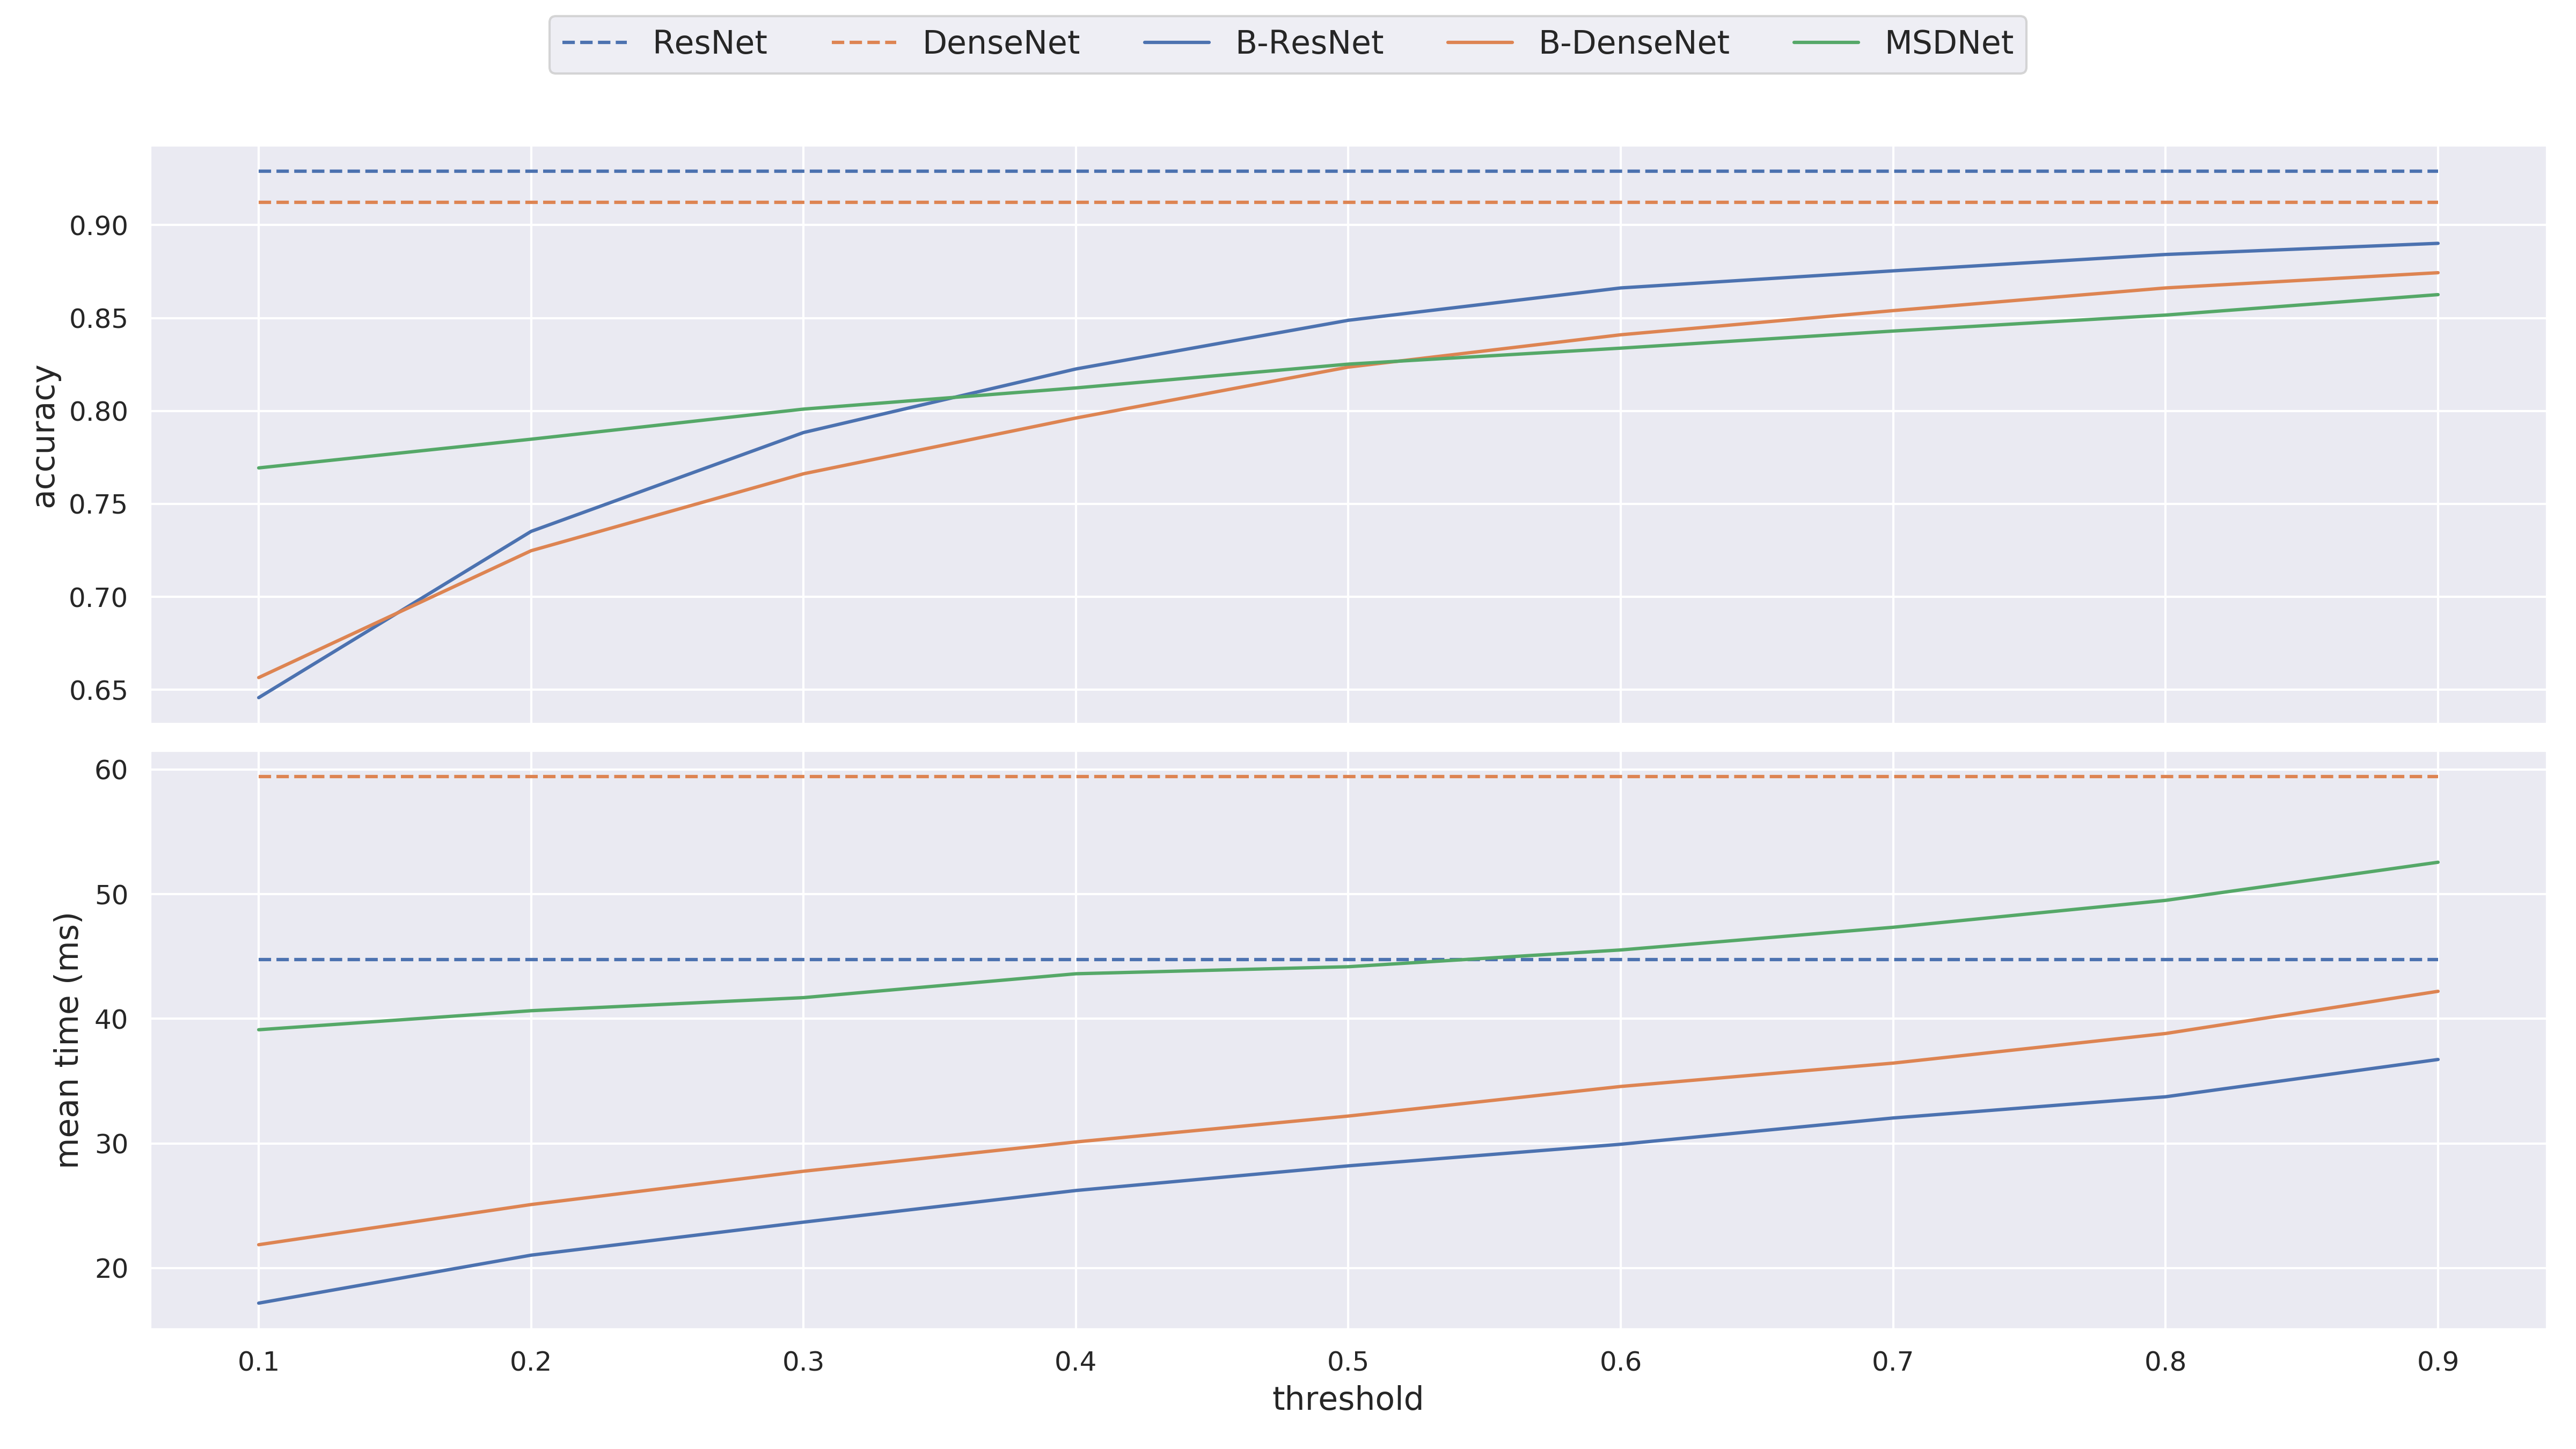
\includegraphics[width=\linewidth]{figures/threshold_plots/compare_exiting_vs_no_exiting}}
  	
  	
  \end{figure}

  \begin{figure}
	\captionsetup[subfigure]{justification=centering}
	\centering
	\subfloat[Jetson TX2\label{fig:jetson-early_exit_vs_conv}]{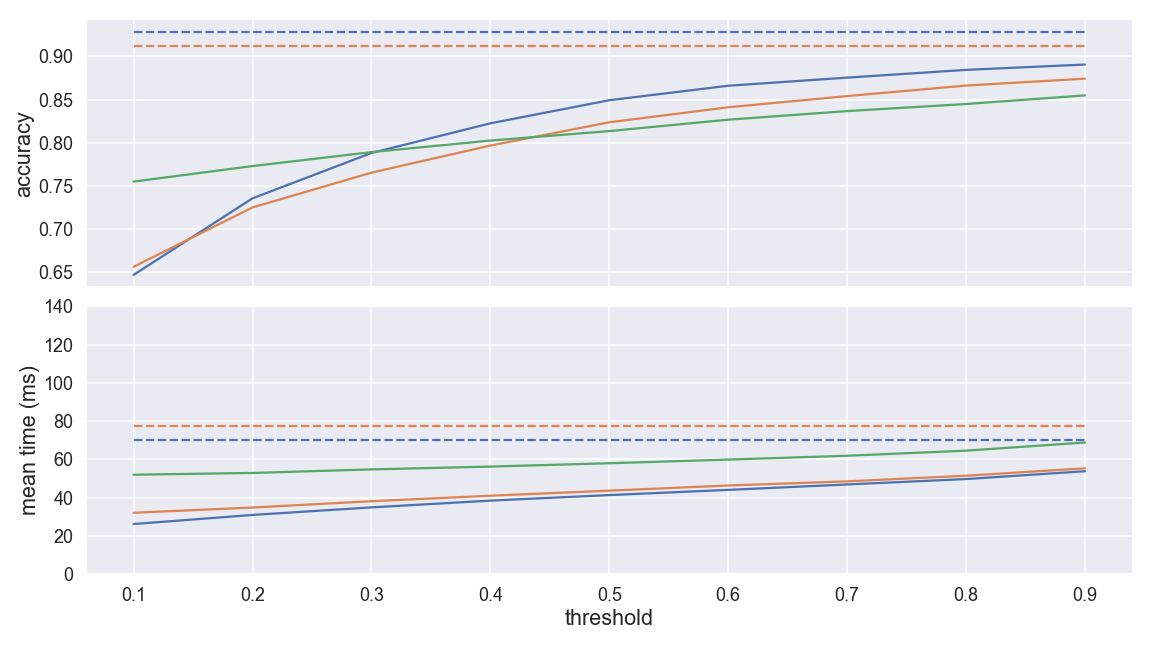
\includegraphics[width=\linewidth]{figures/threshold_plots/jetson_inference}}
\end{figure}

The figure clearly states the accuracy-latency trade-off imposed by early exiting. The conventional models are clearly more accurate, however also expectantly slower, than their more flexible exiting counterpart. B-\gls{densenet} benefits more from early exiting, when a threshold of 0.9 is chosen, it gives up 4 percentage point in accuracy and reducing inference latency by 29 \%. The B-\gls{resnet} have about the same compromise in terms of accuracy, however only a reduction of 18 \% inference latency. B-\gls{resnet} still perform better in terms of both accuracy and inference time. The \gls{resnet}. 

  \begin{figure}
	\captionsetup[subfigure]{justification=centering}
	\centering
	\subfloat[Jetson TX2 fine-grained\label{fig:jetson-fingrained}]{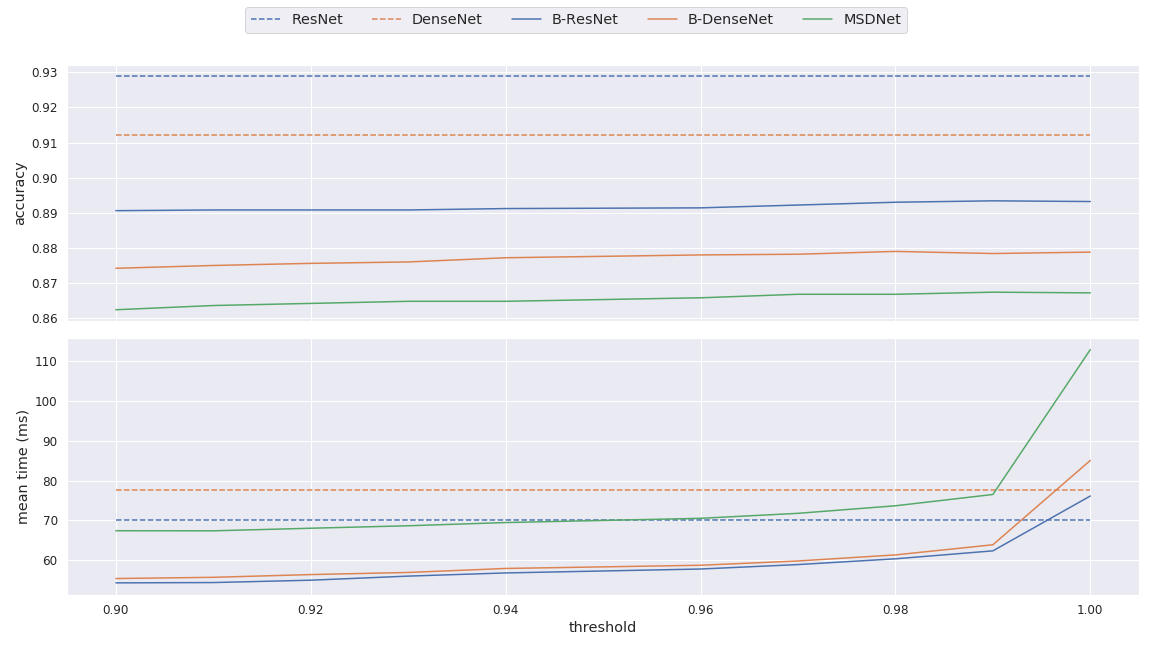
\includegraphics[width=\linewidth]{figures/threshold_plots/jetson_inference_finegrained}}
	\caption[]{}
\end{figure}

\section{Inference Time Analysis}

\begin{figure}
	\captionsetup[subfigure]{justification=centering}
	\centering
	\subfloat[Windows PC]{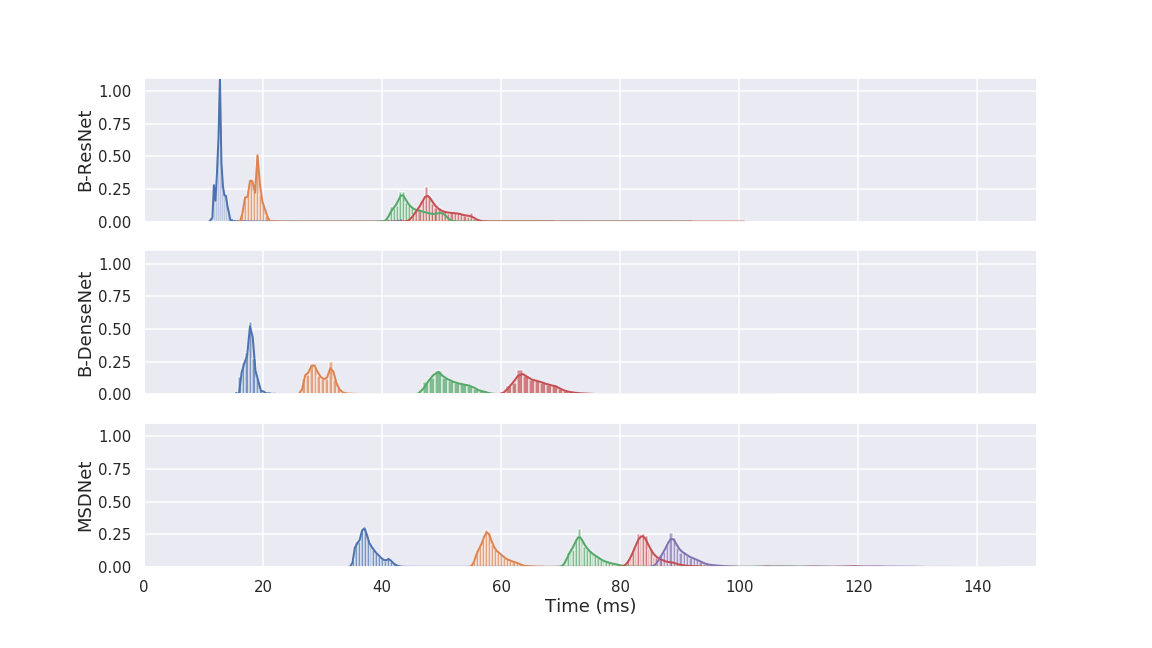
\includegraphics[width=\linewidth]{figures/threshold_plots/inference_time_distribution}}
\end{figure}
\begin{figure}
	\captionsetup[subfigure]{justification=centering}
	\centering
	\subfloat[Jetson TX2]{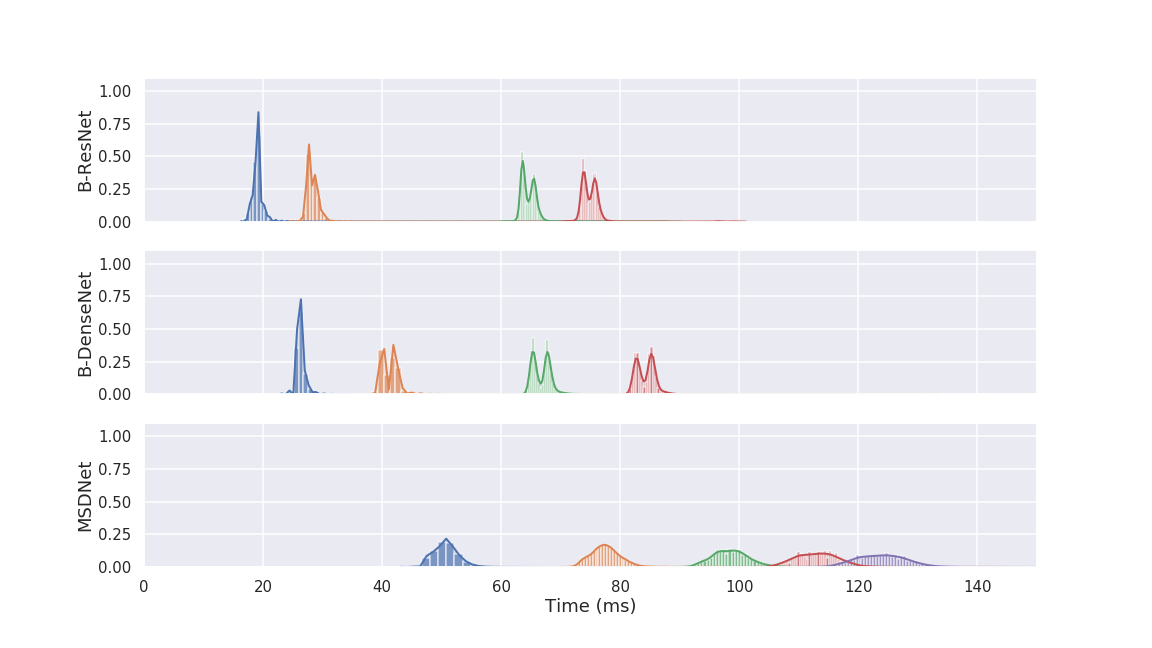
\includegraphics[width=\linewidth]{figures/threshold_plots/jetson_inference_time_distribution}}
	\caption[Inference Time Distribution]{Inference Time Distribution}
\end{figure}

\section{Time Threshold}

\begin{figure}
	\captionsetup[subfigure]{justification=centering}
	\centering
	\subfloat[GPU Workstation]{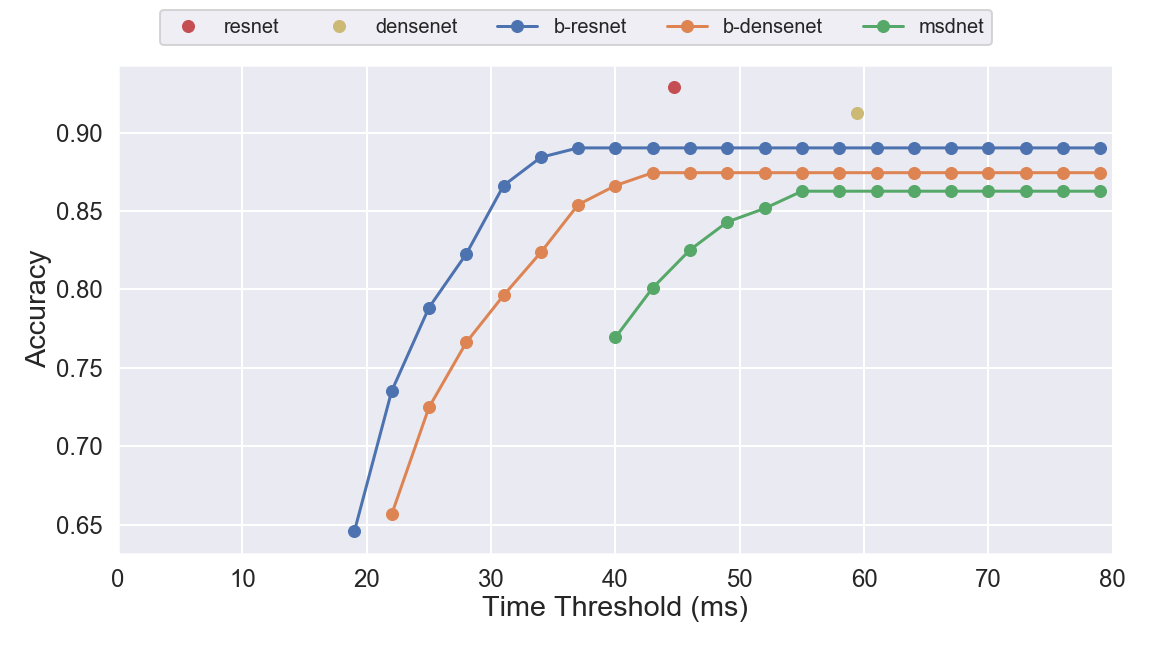
\includegraphics[width=\linewidth]{figures/threshold_plots/time_threshold_pc}}
	\hfill
	\subfloat[Jetson TX2]{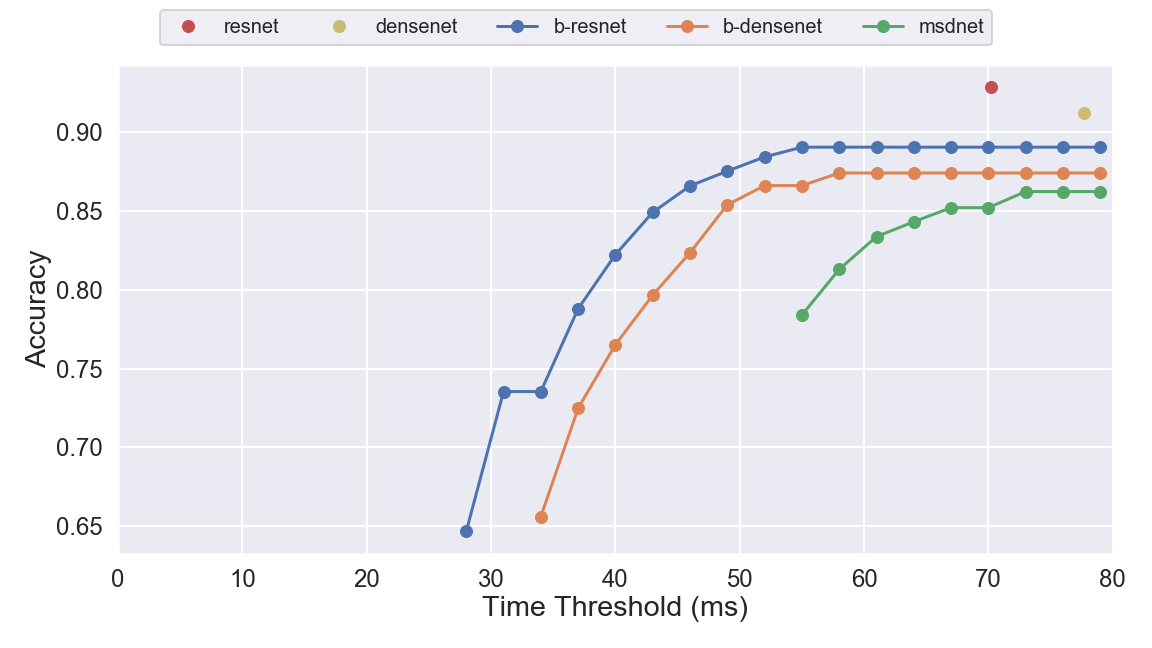
\includegraphics[width=\linewidth]{figures/threshold_plots/time_threshold_jetson}}
	\caption[Time Threshold]{Time Threshold}
\end{figure}

\section{Transport Protocol} 

Offloading tasks over the network, irregardless fully or partially requires a transport protocol. The selection is typically a choice of either \gls{tcp} or \gls{udp}. \gls{tcp} is a reliable protocol, that guarantee no losses by retransmission of lost packets. \gls{udp} on the other hand is a best-effort protocol, that accept packets loss, thus not introducing retransmission communication overhead. 


Fully offloading \gls{jpeg} compressed images for classification require no losses for human-readability. Sending intermediate features of a \gls{dnn} may not be as intolerant to losses and might be able to function with the far more lightweight \gls{udp}. In current research literature the choice of \gls{tcp} seems given in advance.  

In this experiment the \gls{tcp} transmission time and retransmission rate is investigated under different communication environments. 

\begin{figure}
	\centering
	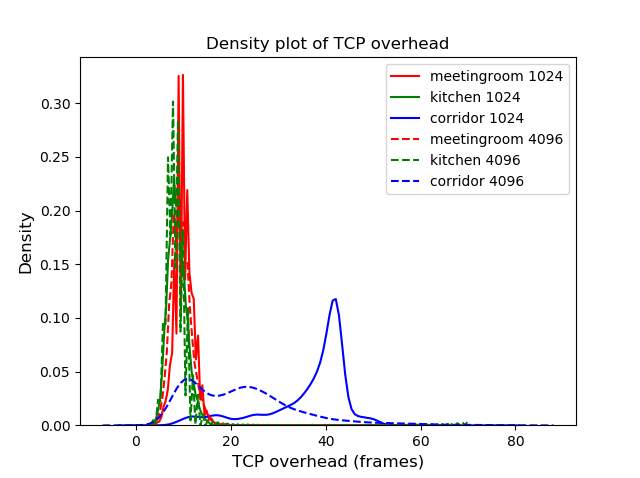
\includegraphics[width=\linewidth]{figures/tcp/tcpoverhead}
	\caption[TCP retransmission overhead]{TCP retransmission overhead}
\end{figure}